\documentclass[12pt,oneside]{report}
\title{{Integrable Systems in Celestial Mechanics}}
\date{September 2024 \\[1cm] {\normalsize{Supervisor: Prof James Lucietti}}}
\author{Abdullah Mohamed Fouzuddeen}
\usepackage[y4project,fancyhdr,hyperref,colour]{edmaths}

% Comment out sections of code
\usepackage{comment}
\usepackage{float}
\usepackage{placeins}

\usepackage[backend=biber,style=numeric,citestyle=numeric]{biblatex}
\addbibresource{references.bib}



% Include the cancel package
\usepackage{cancel}  

% Vector notation package
\usepackage{esvect}

% Format ordinal numbers
\usepackage[super]{nth}

% TikZ for graphics
\usepackage{tikz}
\usepackage{pgfplots}
\usetikzlibrary{arrows.meta}
\usetikzlibrary{decorations.pathmorphing}
\usepackage{subcaption}


% Additional style package
\usepackage{jack}

% Framed environments
\usepackage{mdframed}

% Ensure minimum space before a new section
\usepackage{needspace}

% Define theorem-like environments
\usepackage{amsthm}
% Define theorem styles
\newtheorem{theorem}{Theorem}[section]  % Theorem numbering based on section
\newtheorem{lemma}[theorem]{Lemma}
\newtheorem{corollary}[theorem]{Corollary}
\newtheorem{Proposition}[theorem]{Proposition}

\theoremstyle{definition}
\newtheorem{definition}{Definition}
\newtheorem{question}{Question}
\newtheorem{solution}{Solution}
\newtheorem{example}{Example}
\newtheorem{remark}{Remark}






% Custom math symbols and operators
\newcommand{\df}{\mathrel{\mathop:}=}
\renewcommand{\mod}[1]{\left\lvert #1 \right\rvert}
\renewcommand{\theenumi}{\arabic{enumi}}
\renewcommand{\theenumiii}{\alph{enumiii}}
\renewcommand{\theenumii}{\roman{enumii}}


% Redefine Real and Imaginary parts
\let\Re\relax
\DeclareMathOperator{\Re}{Re}
\let\Im\relax
\DeclareMathOperator{\Im}{Im}
\DeclareMathOperator{\Arg}{Arg}
\DeclareMathOperator{\Log}{Log}

% Partial derivative notation
\newcommand{\dbar}[1]{\frac{\partial #1}{\partial \overline{z}}}
\renewcommand{\d}{\partial}
\renewcommand{\epsilon}{\varepsilon}

% Command for setting size (initialized to 0) changed later
\newcommand{\size}{0}

% Absolute value delimiter
\DeclarePairedDelimiter{\abs}{\lvert}{\rvert}

% Counter for subproofs
\newcounter{subSolutionCounter}[question]

% Custom environment for subproofs
\newenvironment{subsolution}[1][]
    {%
        \vspace{0.3cm}
        \refstepcounter{subSolutionCounter}%
        \par\textbf{Subsolution: \thequestion.\arabic{subSolutionCounter} #1}\par
    }
    {%
        \par% Ensure the paragraph ends
    }

\flushbottom

\begin{document}
\pagenumbering{roman}
\maketitle

\begin{abstract}
The Kepler and Euler problems are special cases of the two-body and three-body problem, respectively. These have been extensively studied by mathematicians such as Euler, Lagrange, Poincaré, and Liouville. In this report, we examine these problems within the broader framework of integrable systems, following Liouville’s integrability criteria from the 18th century. We first introduce the Hamiltonian formulation of mechanics, which leads to the Liouville-Arnold theorem, providing a geometric perspective on phase space trajectories. We then verify the integrability of the Kepler and Euler problems and analyse their explicit solutions, drawing on the reference text Integrable Systems in Celestial Mechanics \cite{o2008integrable}. Finally, we construct the corresponding action-angle variables and compare key differences between the two problems.
\end{abstract}

\declaration

%%\section*{Acknowledgement}

\chapter*{Acknowledgements}
\thispagestyle{empty}
I would like to express my deepest gratitude to my supervisor, Prof.James Lucietti, for his invaluable insight, encouragement, and patience throughout this process. His kindness and support throughout the writing process have meant a great deal to me.

I am also incredibly grateful to my peers and friends for their encouragement during this writing process. In particular, I would like to thank Aiman and Henry for their helpful suggestions, which have greatly contributed to improving this report.

Finally, I extend my heartfelt thanks to my family back home for their unwavering support throughout my academic journey. Their belief in me has been a constant source of strength, and I would not be here without them.

\clearpage

\tableofcontents
\addcontentsline{toc}{chapter}{Contents}
\newpage
\pagenumbering{arabic}


\chapter{Introduction}
 In 1687, Newton solved the two-body problem in his \textit{Philosophi\ae{} Naturalis Principia Mathematica} using purely geometric arguments. In Proposition 66 of Book 1 \cite{linsky1996principia}, he took the first steps toward studying the motion of three bodies under mutual gravitational attraction. Since then, mathematicians and physicists have been captivated by the three-body problem because of its fundamental role in understanding celestial orbits. Despite centuries of study, the three-body problem remains only partially understood. A key difference between the two problems was revealed in the 19th century when Poincar\'e proved that the three-body problem, in general, is non-integrable. This naturally raises the question: what does it mean for a mechanical system to be integrable? At first glance, the answer is not obvious. However, Liouville provided a precise criterion by requiring the existence of a complete set of independent first integrals in involution \footnote{A more precise definition can be seen later see \ref{liouville}.}, a condition that is deeply rooted in the geometry of phase space. In essence, the presence of these integrals implies that the phase space can be foliated into invariant manifolds (typically tori), on which the motion is regular and can be described using action-angle variables. This geometric perspective lies at the heart of our study of integrable systems in celestial mechanics.

Celestial mechanics offers only a few integrable systems. Among these are the Kepler problem (the two-body problem), the Euler problem (the two-fixed-centre problem), and the Vinti problem (a variation of the two-fixed-centre problem). We focus on the Kepler problem and the planar case of the Euler problem. The Kepler problem is a classic example in which two bodies interact through a central force obeying an inverse-square law; one body is fixed at the origin while its gravitational influence on the other is studied. In contrast, the Euler problem involves two fixed bodies whose gravitational influence on a free body forms a variation of the three-body problem. This problem is particularly motivated by its application in modelling satellite orbits around Earth \cite{o2008integrable}. In this model, the two fixed centres are positioned along an axis at imaginary points located at \( \pm ib \) from the origin\footnote{This the aforementioned Vinti problem, more of this can be read in the reference text \cite{o2008integrable}}, leading to analytic formulas that closely approximate the oblate nature of Earth's gravitational field.

In this report, we investigate integrable systems in celestial mechanics with two primary objectives. First, we define what it means for a system to be integrable and examine its properties through the Liouville-Arnold Theorem, emphasizing the deep geometric structure underlying phase space. Second, we apply these concepts to classical problems, drawing guidance from \cite{o2008integrable} to construct explicit solutions.

\begin{itemize}
    \item \textbf{Chapter 2} develops a foundation in Hamiltonian mechanics and introduces the essential tools and background necessary to appreciate the geometric nature of phase space.
    \item \textbf{Chapter 3} explores the Kepler problem, proving the integrability criteria, deriving explicit solutions, and constructing the corresponding action-angle variables via the Liouville-Arnold Theorem.
    \item \textbf{Chapter 4} examines the planar Euler problem, exploring its non-trivial geometric structure through Möbius transforms and Jacobi elliptic functions to solve for trajectories. We then construct action-angle variables for the Euler problem and compare them with the Kepler case.
\end{itemize}

This report assumes that the reader is comfortable with Lagrangian mechanics and familiar with differential geometry. For clarity, we also outline the key influences on this work and highlight our own contributions.
\begin{itemize}
    \item \textbf{Chapter 2} draws from multiple sources, particularly \cite{arnol2013mathematical}, \cite{goldstein2002classical}, \cite{TMPB23/24} and \cite{DavidTong}.
    \item \textbf{Chapter 3} presents an original discussion on integrability criteria and Hamiltonian formulation, while the sections on trajectories follow \cite{o2008integrable}. The construction of action-angle variables was aided by \cite{goldstein2002classical}.
    \item \textbf{Chapter 4} follows \cite{o2008integrable} for trajectory solutions. However, our discussion on coordinate choices, integrability, and action-angle variables is entirely original. To our knowledge, the final result is not explicitly available in existing literature. The plots and Mathematica code provided in this chapter were created by us (see Appendix \ref{Mathematica code}).
\end{itemize}

 




\chapter{Classical Mechanics and Symplectic Geometry}
Before discussing integrable systems, it's worth reviewing the formalisms used. We'll start by briefly reminding ourselves of some key ingredients in the Lagrangian framework and why it's considered useful, followed by a brief introduction to the Hamiltonian formulation. It's also important to understand the methods used to approach these mechanical problems. We explore these methods and the geometric context at the end of the chapter. This chapter is based on various sources, particularly \cite{arnol2013mathematical}, \cite{goldstein2002classical}, \cite{TMPB23/24}, and \cite{DavidTong}.



\section{Hamiltonian Mechanics}


\begin{definition}[Lagrangian and Action]\label{Definition 1}
Consider a system with generalized coordinates $\mathbf{q} \in \mathbb{R}^{n}$ and velocities $\dot{\mathbf{q}} \in \mathbb{R}^{n}$, with kinetic energy $T$ and potential energy $V$, and assume a time-independent Lagrangian\footnote{We are only concerned with time-independent Lagrangians in this report and will make this simplification where possible.}. The Lagrangian is a smooth function $
\mathcal{L} : \mathbb{R}^{2n} \to \mathbb{R}$, sending $ (\mathbf{q},\dot{\mathbf{q}}) \mapsto \mathcal{L}(\mathbf{q},\dot{\mathbf{q}}) 
$. The action functional associated to $\mathcal{L}$ is defined as
\[
S[\mathbf{q}] = \int_{t_0}^{t_1} \mathcal{L}(\mathbf{q},\dot{\mathbf{q}})\,dt,
\]
where the Lagrangian function is defined as

\begin{equation}\mathcal{L}(\mathbf{q},\dot{\mathbf{q}}) = T-V\end{equation}
and $t_0, t_1 \in \mathbb{R}$ denote the initial and final times, respectively.
\end{definition}

\noindent A fundamental result in the Lagrangian formalism is given by the Euler-Lagrange theorem.
\begin{theorem}[Euler-Lagrange]\label{Theorem Euler-Lagrange}
    The extremals of the action functional in Definition \ref{Definition 1} satisfy the Euler-Lagrange equations, given by \autoref{Euler Lagranges Equations} for $i \in \{1,\cdots n\}$.
    \begin{equation} \label{Euler Lagranges Equations}
        \td{}{t} \left( \pd{\mathcal{L}}{\dot{q_{i}}} \right) = \pd{\mathcal{L}}{q_{i}} 
    \end{equation}
\end{theorem}

\noindent Having established the key terminology, we now illustrate these concepts with an example.

\begin{example}\label{example 1}
    Consider a conserved mechanical system with mass $m$ and potential $V(\textbf{x})$ in $\R^{3}$. The Lagrangian function would be defined as follows,
    \begin{equation}
        \mathcal{L} = \frac{m}{2}\sum_{i=1}^{3}\dot{x}_{i}^{2} - V(\textbf{x})
    \end{equation}
   Applying the Euler-Lagrange equations to the above Lagrangian for the $x_{i}^{\textit{th}}$ (the $i^{\textit{th}}$ component of $\textbf{x}$)
  coordinate, we obtain
    $$ m\ddot{x}_{i} = -\pd{V}{x_{i}}$$
    which is $i^{\textit{th}}$ component of Newton's $2^{\textit{nd}}$ law for the system. ($ \textbf{F} = m\ddot{\textbf{x}}$ where, $\textbf{F} = -\underline{\nabla} V$). 
\end{example}

This highlights the advantages of Lagrangian mechanics, as it provides an equivalent formulation to Newton’s laws while allowing for a more convenient coordinate choice without the complexities of the vectorial approach used in Newtonian mechanics. Now that we're familiar with the formulation we can start discussing the Hamiltonian formalism.

\begin{definition}[Hamiltonian]\label{Hamiltonian}
    Given an explicit, time-independent Lagrangian function $\mathcal{L}(\textbf{q}, \dot{\textbf{q}})$ we define the Hamiltonian function as
    \begin{equation}\label{Def_Ham}
        H(\textbf{q},\textbf{p}) = \sum_{i} p_{i} \dot{q_{i}} - \mathcal{L}(\textbf{q}, \dot{\textbf{q}}).
    \end{equation}
    This is a smooth function, $H:\R^{2n} \rightarrow \R $, where $\textbf{q}$ and $\textbf{p}$ denote the generalised coordinates and momenta of the system. The $i^{\textit{th}}$ generalised momentum $p_{i}$ is defined via the Lagrangian as
    $$ p_{i} \defequal \pd{\mathcal{L}}{\dot{q_{i}}} .$$
    Hamilton's equations are defined as follows
    \begin{equation} \label{1.4}
 \pd{H}{p_{i}} = \dot{q_{i}}  \ , \ \pd{H}{q_{i}} = -\dot{p_{i}}. \    
\end{equation} 
\end{definition}

\noindent It's useful at this stage to consider an example of this formulation.

\begin{example}
    The Hamiltonian for a conserved mechanical system with mass $m$ and potential $V(\textbf{x})$ in $\R^{3}$ reads as
    \begin{equation}
        H = \frac{1}{2m}\sum_{i=1}^{n} p_{i}^{2}+V(\textbf{x}).
    \end{equation}
    Hamilton's equation now gives
    $$ \frac{p_{i}}{m} = \dot{x_{i}}  \ , \ \pd{V}{x_{i}} = -\dot{p}_{i}.$$
    Putting this together we get
    $$ m\ddot{x}_{i} = -\pd{V}{x_{i}}.$$
    This result recovers Newton's second law and is consistent with the Euler-Lagrange equations, as expected.
\end{example}

\begin{theorem}
  Suppose the system is mechanical and the kinetic energy is of quadratic with respect to $\dot{\textbf{q}}$, then the Hamiltonian $H$ is the total energy of the system  
\end{theorem}
\begin{proof}
 Recall that the Hamiltonian is defined as Definition \ref{Hamiltonian},
$$  H(\textbf{q},\textbf{p}) = \sum_{i} p_{i} \dot{q_{i}} - \mathcal{L}(\textbf{q}, \dot{\textbf{q}})$$
since kinetic energy is quadratic with respect to  $\dot{\textbf{q}}$, $T$ takes the form
$$  T = \cfrac{1}{2} \sum_{i,j}a_{ij}\dot{q}_{i}\dot{q}_{j},$$
where $a_{ij} = a_{ij}(\textbf{q})$, now $p_{i}$ have the form\
%%NB: use a different index+ product rule to avoid confusion!
$$ p_{i} = \pd{\mathcal{L}}{\dot{q}_{k}} =  \sum_{i,k}a_{ik}\dot{q}_{i} ,$$
thus the Hamiltonian now reads
$$ H =  \sum_{i,j}a_{ij}\dot{q}_{j}\dot{q_{i}} - \mathcal{L}(\textbf{q}, \dot{\textbf{q}}) = 2T - \mathcal{L}$$
$$  H = 2T-(T-V) = T+V .$$

\end{proof}
\noindent This underlies the physical interpretation of the Hamiltonian function as the total energy of a mechanical system.
\begin{definition}
   A coordinate $q_{1}$ is said to be cyclic if it does not appear explicitly in the Hamiltonian, i.e., i.e $\d H/\d q_{1} =0$. 
\end{definition}
\noindent An immediate consequence of a cyclic coordinate is that its corresponding conjugate momenta is a constant of motion this follows directly from Hamilton's equations.

While the Hamiltonian formalism reduces the order of the differential equations from $n$ second-order ODEs to $2n$ first-order ODEs (where
$n$ is the number of degrees of freedom), it also increases the total number of equations. In practice, while this does not make it easier to solve problems, we gain much more conceptually and structure-wise. One such example is the Poisson bracket structure.

\subsection{Poisson Bracket}
The Poisson bracket is an operation on smooth functions on phase space \footnote{Phase space is given a mathematical definition later in terms of the cotangent bundle see \ref{Symplectic geometry sec}. For now one can just assume its equivalent to $\R^{2n}$ where it is the space of position and momenta.} defined as follows.
\begin{definition}\label{poisson bracket}
    Let $f(\textbf{q},\textbf{p})$ and $g(\textbf{q},\textbf{p})$ be smooth functions on phase space. Then the Poisson bracket is given by
    $$ \left\{f,g \right\}  \defequal \sum_{i} \pd{f}{q_{i}}\pd{g}{p_{i}} - \pd{g}{q_{i}}\pd{f}{p_{i}} .$$
\end{definition}
\begin{Proposition}
    Let $f,g,h$ be smooth functions on phase space and $\alpha,\beta \in \R$, then the Poisson bracket satisfies the following properties:
    \begin{enumerate}
        \item Skew-symmetry: \ $ \pb{f}{g} = -\pb{g}{f}$
        \item Linear in its entries in $\R$ : \ $\pb{\alpha f + \beta g}{h} = \alpha \pb{f}{h} + \beta \pb{g}{h}$
        \item Leibniz rule : \  $\pb{fg}{h} = f \pb{g}{h} + \pb{f}{h} g$
        \item Jacobi identity : $\pb{f}{\pb{g}{h}} + \pb{g}{\pb{h}{f}} + \pb{h}{\pb{f}{g}} = 0 $
    \end{enumerate}
\end{Proposition}

\begin{proof}
   \begin{enumerate}
       \item $ \pb{f}{g} = \sum_{i} \pd{f}{q_{i}}\pd{g}{p_{i}} - \pd{g}{q_{i}}\pd{f}{p_{i}} = \sum_{i} \pd{g}{q_{i}}\pd{f}{p_{i}} -\pd{f}{q_{i}}\pd{g}{p_{i}} = -\pb{g}{f}.  $
       \item This follows from linearity of the partial derivative.
       \item This follows from the Leibniz rule for partial derivatives.
       \item It follows from straightforward expansion of the expression.
   \end{enumerate} 
\end{proof}


\noindent The Poisson bracket plays a fundamental role in Hamiltonian mechanics, as seen in the following propositions.


\begin{Proposition}\label{pbrel}
    Let $f$ be a smooth function on phase space then
   $$ \td{f}{t}  = \pb{H}{f} +\pd{f}{t} .$$
\end{Proposition}

\begin{proof}
$f$ is a smooth function on phase space thus
$$\td{f}{t} = \sum_{i}\pd{f}{q_{i}}\dot{q_{i}}+ \pd{f}{p_{i}}\dot{p_{i}} + \pd{f}{t}.$$
Using Hamilton's equations we obtain
$$ =  \sum_{i}\pd{f}{q_{i}}\pd{H}{p_{i}} - \pd{f}{p_{i}}\pd{H}{q_{i}} +\pd{f}{t}$$
$$  \td{f}{t}= \pb{f}{H} + \pd{f}{t}.$$
    
\end{proof}
An immediate consequence of this is the fact that Hamilton's equation can be  rewritten in terms of the Poisson bracket as follows
$$ \td{q_{i}}{t}=\pb{q_{i}}{H} \ , \ \td{p_{i}}{t}=\pb{p_{i}}{H}.$$

\begin{Proposition}
    Let $I$ be a smooth function on phase space that does not depend explicitly on time. $I$ is a constant of motion (i.e. $\frac{dI}{dt}=0$) if and only if
    \[
    \{I,H\} = 0.
    \]
\end{Proposition}

 \begin{proof}
     Since $I$ is a constant of motion with no explicit time dependence, it follows from Proposition \ref{pbrel} that
     $$\td{I}{t} = 0 \implies \pb{I}{H} + \pd{I}{t} = 0$$
     since there is no explicit time dependence
     $$ \pb{I}{H} = 0.$$
    the argument works both ways as required.
 \end{proof}

\noindent The Poisson bracket provides a powerful tool for identifying conserved quantities and plays a crucial role in integrable systems, as we will explore later.
\begin{remark}
 We may use the following terminology that if $\pb{I}{H} = 0 $, then $I$ and $H$ are in involution.    
\end{remark}

Before proceeding, we establish some fundamental Poisson bracket identities that will be useful for later calculations.
\begin{Proposition}\label{useful id}
    Let $p_{i}$ and $q_{i}$ be the generalised momenta and coordinates respectively then the following identity holds with $\pb{.}{.}$ 
    $$\pb{q_{i}}{q_{j}} = 0 \ , \ \pb{p_{i}}{p_{j}} = 0 \ , 
    \ \pb{p_{i}}{q_{j}} = \delta_{ij}$$
\end{Proposition}
\begin{proof}
    This follows from the definition of the Poisson brackets.
\end{proof}

\section{Hamilton-Jacobi Theory and Action-Angle Variables}
In this section, we introduce a key technique in Hamiltonian mechanics that allows us to analyse phase space trajectories by determining periodic motion frequencies. This is achieved through action-angle variables, which provide insight without requiring explicit trajectory solutions. In later chapters, we shall use these techniques to understand a few problems in detail. We begin by identifying transformations that preserve the structure of Hamilton's equations and justify a specific transformation that renders the Hamiltonian cyclic with respect to a new set of coordinates.
\subsection{Canonical Transformations}
A key feature of the Lagrangian formulation is that the equations of motion remain invariant under changes in generalised coordinates. In this section, we identify the transformations in Hamiltonian mechanics that preserve this property. To do so, we first introduce a method for simultaneously handling Hamilton's equations. Let 
$
\mathbf{x} =
    \begin{pmatrix}
           q_{1}, 
            \cdots, 
           q_{n}, 
           p_{1}, 
           \cdots, 
           p_{n}
    \end{pmatrix}^{T},
$
Hamilton’s equations can then be rewritten as follows:
\begin{equation} \label{symHam}
 \dot{\mathbf{x}} = \Omega\frac{\partial H}{\partial \mathbf{x}}  \quad \text{or} \quad \dot{x}_{i} = \Omega_{ij} \frac{\partial H}{\partial x_{j}},
\end{equation} 
where $\Omega$ is a $2n \times 2n$ matrix of the form,
\begin{equation}
 \Omega = 
\begin{bmatrix}\label{symplectic}
\mathbf{0}_{n \times n} & I_{n \times n} \\
-I_{n \times n} & \mathbf{0}_{n \times n}
\end{bmatrix}.   
\end{equation}

%\begin{remark}
 % One may recognize this as the symplectic form on the vector space $\mathbb{R}^{2n}$.
%\end{remark}

Now we seek a transformation $\mathbf{x} \rightarrow \mathbf{y}$ that keeps Hamilton's equations invariant, i.e.,
\[
\dot{y}_{i} = \Omega_{ij} \frac{\partial H}{\d y_{j}}.
\]
The relation between $\dot{y}_{i}$ and $\dot{x}_{l}$ is given by
\[
\dot{y}_{i} = \frac{\partial y_{i}}{\partial x_{l}} \dot{x}_{l},
\]
then using \autoref{symHam}, we obtain
\[
\dot{y}_{i} = \frac{\partial y_{i}}{\partial x_{l}} \Omega_{lm} \frac{\partial H}{\d x_{m}} = \frac{\partial y_{i}}{\partial x_{l}} \Omega_{lm} \frac{\partial H}{\d y_{j}} \frac{\partial y_{j}}{\partial x_{m}}.
\]
Thus, the transformation preserves Hamilton's equation if
\[
\Omega_{ij} = \mathcal{J}_{il} \Omega_{lm} \mathcal{J}^{T}_{mj},
\]
where $\mathcal{J}_{il} = \frac{\partial y_{i}}{\partial x_{l}}$ is the Jacobian matrix. This motivates the following definition.
\begin{definition}[Canonical transformations]
  A change of coordinates in phase space $\textbf{x} \rightarrow \textbf{y}$ is called a canonical transformation if the Jacobian matrix $\mathcal{J}$ obeys $$\mathcal{J}\Omega\mathcal{J}^{T} = \Omega$$ 
  and then the Jacobian matrix $\mathcal{J}$ is called symplectic. \end{definition}



\begin{Proposition}
    The Poisson bracket is invariant under canonical transformations. 
\end{Proposition}
\begin{proof}
    Consider the smooth functions $f(\textbf{x}),g(\textbf{x})$ on phase space then the Poisson bracket of $f$ and $g$ is given by
    $$\pb{f}{g} = \sum_{i} \left( \pd{f}{q_{i}}\pd{g}{p_{i}}-\pd{f}{p_{i}}\pd{g}{q_{i}} \right),$$
    or using the notation above
    $$\pb{f}{g} = \pd{f}{x_{i}}\Omega_{ij}\pd{g}{x_{j}}.$$
    Under a transformation $\textbf{x} \rightarrow \textbf{y}(\textbf{x})$ we obtain
    $$  \pd{f}{x_{i}} = \pd{f}{y_{k}}\mathcal{J}_{ki},$$
    $$\pb{f}{g} = \pd{f}{y_{k}}\mathcal{J}_{ki}\Omega_{ij}\mathcal{J}_{lj}\pd{g}{y_{l}} = \pd{f}{y_{k}}\Omega_{kl}\pd{g}{y_{l}}$$
        where the final equality is because the transformation is symplectic. Therefore
    $$  = \pb{f(\textbf{y})}{g(\textbf{y})}.$$

\end{proof}

\begin{Proposition}
 The converse statement is also true, if the Poisson bracket structure is conserved such that $$ \pb{Q_{i}}{Q_{j}} = 0 \ , \pb{P_{i}}{P_{j}} = 0 \ , \ \pb{Q_{i}}{P_{j}} = \delta_{ij},$$ where ${P_{i}},{Q_{i}}$ are the new coordinates which were represented as $\textbf{y}$. Then $\textbf{x} \rightarrow \textbf{y}$ is a canonical transformation, where $\textbf{x}$ is the old-coordinates.    
\end{Proposition}

Having established that symplectic transformations preserve the structure of Hamiltonian mechanics, we now introduce a systematic way to construct these transformations: generating functions. These functions allow us to transition between coordinate systems while ensuring that the new equations of motion remain Hamiltonian.

Let $  (q_{i}, p_{i}) $ be the original phase-space coordinates, and define the new coordinates $ (Q_{i}, P_{i}) $ via an invertible transformation:
$$ Q_i \coloneqq Q_i(q_i, p_i), \quad P_i \coloneqq P_i(q_i, p_i).
$$
If there exists a function $ K(\textbf{Q}, \textbf{P}) $ (the Hamiltonian for the new coordinate system) such that Hamilton's equations hold:
$$
\dot{Q}_i = \frac{\partial K}{\partial P_i}, \quad \dot{P}_i = -\frac{\partial K}{\partial Q_i},
$$
then we say \( (Q_i, P_i) \) form a canonical coordinate system. Since we are interested in a canonical transformation from the old set of coordinates $(q_{i},p_{i})$ to $(Q_{i},P_{i})$, we require that the equations of motion coincide we shall do this via the action \footnote{We've already shown by way of an example Hamilton's equations and the Euler-Lagrange equations are equivalent for conserved mechanical systems.}. Recall Definition \ref{Hamiltonian} of the Hamiltonian via the Lagrangian:
$$
H(\textbf{q}, \textbf{p}, t) = \sum_{i} p_i \dot{q}_i - \mathcal{L}(\textbf{q}, \dot{\textbf{q}}, t),
$$
which gives the action functional:
$$
S = \int_{t_0}^{t_1} \mathcal{L}(\textbf{q}, \dot{\textbf{q}}, t) \, dt = \int_{t_0}^{t_1} \left(\sum_{i} p_i \dot{q}_i - H(\textbf{q}, \textbf{p}, t)\right) dt.
$$
The transformation is canonical if the new action
$$
S' = \int_{t_0}^{t_1} \left(\sum_{i} P_i \dot{Q}_i - K(\textbf{Q}, \textbf{P}, t)\right) dt
$$
leads to equivalent equations of motion, i.e., 
$$\delta S = \delta S' = 0.$$

To ensure that the new and old coordinate systems yield equivalent equations of motion, we introduce an appropriate generating function 
 $F$ that satisfies the condition:
\begin{equation}\label{genfn}
    \sum_{i}p_{i}\dot{q}_{i} - H(\textbf{q},\textbf{p},t) = \sum_{i}P_{i}\dot{Q}_{i} - K(\textbf{Q},\textbf{P},t) + \td{F}{t}
\end{equation}

where $F$ is any function of the phase space coordinates as variation of the path are zero at the end points (i.e $\delta Q_{i}=\delta P_{i}=0$ and $\delta p_{i} = \delta q_{i} =0$ ). While there are 4 types of generating functions we focus on what's usually referred to as $F_{1}$ in the literature \cite{goldstein2002classical}, where explicitly
$$ F = F_{1}(\textbf{q},\textbf{Q},t).$$
We consider the case that $q_{i}$ cannot be expressed as a function of $Q_{i}$ and $t$; if this is not the case, a different generating function should be used. From \autoref{genfn} we get the relation
$$\sum_{i}p_{i}\dot{q}_{i}-H =\sum_{i} \left(P_{i}\dot{Q}_{i}-K+\pd{F_{1}}{q_{i}}\dot{q}_{i}+\pd{F_{1}}{Q_{i}}\dot{Q}_{i}+\pd{F_{1}}{t} \right)$$
$$= \sum_{i}\left(-K+\pd{F_{1}}{q_{i}}\dot{q}_{i}+\pd{F_{1}}{Q_{i}}\dot{Q}_{i}+\pd{F_{1}}{t}+{P}_{i}\dot{Q}_{i} \right)$$

since the variations of $\dot{q}_{i}$ and $\dot{Q}_{i}$ are independent, the coefficients must match. Comparing the coefficients of $\dot{q}_{i}$ and $Q_{i}$ gives
\begin{equation} \label{Generating function}
 p_{i} = \pd{F_{1}}{q_{i}} \ , \ P_{i} = -\pd{F_{1}}{Q_{i}},   
\end{equation} 
 thus we get the defining relationship between the Hamiltonian functions $K$ and $H$ as
\begin{equation}
    K = H + \pd{F_{1}}{t}.
\end{equation}
In fact one can check these equations ensure that the new coordinates $(Q_{i},P_{i})$ preserve Poisson bracket structure and thus are canonical. 


%one can check this explicitly,
%$$ \pb{Q_{i}}{Q_{j}} = \sum_{k}\pd{Q_{i}}{q_{k}}$$ time and space permitiing ! %%



\subsection{Hamilton-Jacobi Equation and Action-Angle Variables}
We now examine a specific class of canonical transformations using the generating function $F_{1}$ to map from $(q_{i},p_{i}) $ to $ (Q_{i}, P_{i})$. In particular, we seek a transformation where Hamilton’s equations in the new coordinates take the form $K(\textbf{Q},\textbf{P},t) = 0$, i.e. $Q_{i}$ and $P_{i}$ are constants of motion throughout phase space leading to the equations
\begin{subequations} \begin{equation} \label{genHam} \pd{K}{Q_{i}} = \pd{K}{P_{i}} = 0 \implies Q_{i} = \alpha_{i} \in \R, \quad P_{i} = \beta_{i} \in \R. \end{equation} \begin{equation}\label{H-J eqn} H\left(q_{i},\pd{F_{1}}{q_{i}},t \right) + \pd{F_{1}}{t} = 0. \end{equation} \end{subequations}


In \autoref{H-J eqn}, we make use of the relationship established by the generating function \autoref{Generating function}. Due to historical conventions, this specific function $F_{1}(\textbf{q},\textbf{Q},t)$ is often referred to as "Hamilton's principle function", which we will denote as $S$. The \autoref{H-J eqn} is then recognised as the Hamilton-Jacobi equation. To illustrate its application, we consider an explicit example.

\begin{example}\label{SHO}
Consider a one dimensional simple harmonic oscillator (SHO) with unit mass and frequency $\omega$. The Hamiltonian is given by
\begin{equation}
H(q,p) = \frac{1}{2} p^{2} + \frac{1}{2} \omega^{2} q^{2}.
\end{equation}
Using the relation from \autoref{Generating function},
\begin{equation}
p = \pd{S}{q}.
\end{equation}
The Hamilton-Jacobi equation takes the form
\begin{equation}
\frac{1}{2} \left(\pd{S}{q}\right)^{2} + \frac{1}{2} \omega^{2} q^{2} + \pd{S}{t} = 0.
\end{equation}
Then we assume the standard separability ansatz 
\begin{equation}
S(q, \alpha, t) = S_q(q) + S_t(t),
\end{equation}
where $Q = \alpha \in \mathbb{R}$, as defined in \autoref{genHam}. Substituting this into the Hamilton-Jacobi equation, we obtain
\begin{equation}
\frac{1}{2} \left(\pd{S_q}{q}\right)^{2} + \frac{1}{2} \omega^{2} q^{2} = -\pd{S_t}{t}.
\end{equation}
Since both sides must equal a constant, we define this constant as $\alpha$, leading to the two ordinary differential equations:
\begin{equation}
\td{S_t}{t} = -\alpha,
\end{equation}
\begin{equation}
\frac{1}{2} \left(\pd{S_q}{q}\right)^{2} + \frac{1}{2} \omega^{2} q^{2} = \alpha.
\end{equation}
Integrating the first equation gives
\begin{equation}
S_t = -\alpha t + C_0.
\end{equation}
We leave $S_q$ in its implicit form for convenience. Combining these results, the solution for $S$ is
\begin{equation}
S(q, \alpha, t) = \int \sqrt{2 \left(\alpha - \frac{1}{2} \omega^{2} q^{2} \right)} \ dq - \alpha t + C_0.
\end{equation}
Using \autoref{Generating function}, the new generalised momentum $P$ is given by
\begin{equation}
P = -\pd{S}{\alpha} = -\frac{1}{\sqrt{2}} \int \frac{dq}{\sqrt{\alpha - \frac{1}{2} \omega^{2} q^{2}}} + t.
\end{equation}
Evaluating the integral, we find
\begin{equation}
P = -\frac{1}{\omega} \arcsin \left( q \frac{\omega}{\sqrt{2\alpha}} \right) + t.
\end{equation}
By definition, $P$ is a constant, which we denote as $\beta \in \mathbb{R}$. Solving for $q(t)$, we have:
\begin{equation}
q(t) = \frac{\sqrt{2\alpha}}{\omega} \sin \omega (t - \beta),
\end{equation}
which is the well-known solution for the simple harmonic oscillator. Notably, $\alpha$ corresponds to the energy of the system, since the Hamiltonian $H$ is a conserved quantity. Similarly, solving for $p$ using \autoref{Generating function}, we obtain
\begin{equation}
p(t) = \sqrt{2\alpha} \cos \omega (t - \beta).
\end{equation}
\end{example}
This example illustrates the key idea behind Hamilton-Jacobi theory it reformulates Hamilton’s equations originally a set of ordinary differential equations (ODEs) into a single partial differential equation (PDE). While this is not always practically useful, it plays a crucial role in the derivation of action-angle variables, as we will see in the following chapters.

Before proceeding, we simplify the Hamilton-Jacobi equation for time-independent Hamiltonians.
\begin{Proposition}\label{Time independent HJ}
    If $H$ is time independent Hamiltonian for a system and $S$ is Hamilton's principle function. Then the Hamilton-Jacobi equation simplifies to,
    $$H\left( q,\pd{W}{q}\right) = E \ \ ,\text{where} \ S = W(Q,q) -tE$$
    and E is the total energy of the system.
\end{Proposition}
\begin{proof}
    Since $\pd{H}{t} = 0 ,$ we recall the identity from proposition \ref{pbrel}
    $$ \td{H}{t} = \pb{H}{H} + \pd{H}{t } = 0,$$
    this implies that $H$ is a conserved quantity, i.e., $H = E$. Substituting the ansatz $S = W(Q,q)+S_{t}$ into Hamilton-Jacobi equation, we obtain
    $$ E+\pd{S_{t}}{t} = 0.$$
    Thus $S_{t} = -Et$  (upto to an integration constant). Therefore, we arrive at the result
    $$S = W(Q,q)-Et,$$
   where $W$ is known as Hamilton's characteristic function, that satisfies the time independent Hamilton-Jacobi equation.
\end{proof}

We now turn our attention to a specific type of canonical transformation central to this report, the action-angle variables. To motivate this transformation, we revisit the example of the simple harmonic oscillator (SHO) and consider the change of variables from $(q, p) \to (\theta, I)$. Recall the solution for the SHO:
$$q(t) = \frac{\sqrt{2\alpha}}{\omega} \sin(\omega(t - \beta)), \quad p(t) = \sqrt{2\alpha} \cos(\omega (t-\beta)). $$

We define the new angle variable $\theta = \omega (t - \beta)$ and the action variable $I = \alpha$. To verify that this transformation is canonical, we compute the Poisson bracket $\pb{q}{p}$:
$$\pb{q}{p} = \frac{\partial q}{\partial \theta} \frac{\partial p}{\partial I} - \frac{\partial q}{\partial I} \frac{\partial p}{\partial \theta} = \left\{\frac{\sqrt{2I}}{\omega} \sin(\theta), \sqrt{2I\omega} \cos(\theta)\right\}, $$
simplifying, we obtain
$$ 2 \{ \sqrt{I} \sin(\theta), \sqrt{I} \cos(\theta) \} = 1. $$ Since the Poisson bracket is preserved, this confirms that the transformation is canonical. Having established this, we now examine the Hamiltonian in terms of the new variables $(I, \theta)$:

$$ H(I,\theta) = \omega I. $$ 
This reveals the key insight, eliminating the dependence on the angle coordinate $\theta$ the Hamiltonian becomes cyclic in $\theta$, effectively "straightening" the flow lines in phase space. A visual representation of this transformation is shown in Figure \ref{flow lines action}. A natural question arises, can such a transformation always be performed ? In general, the answer is no. However, for a special class of systems known as integrable systems, such a transformation is possible. This will be discussed in more detail in the following section. For now let us define the action variable in one dimension.
\begin{figure}[htbp]
    \centering
    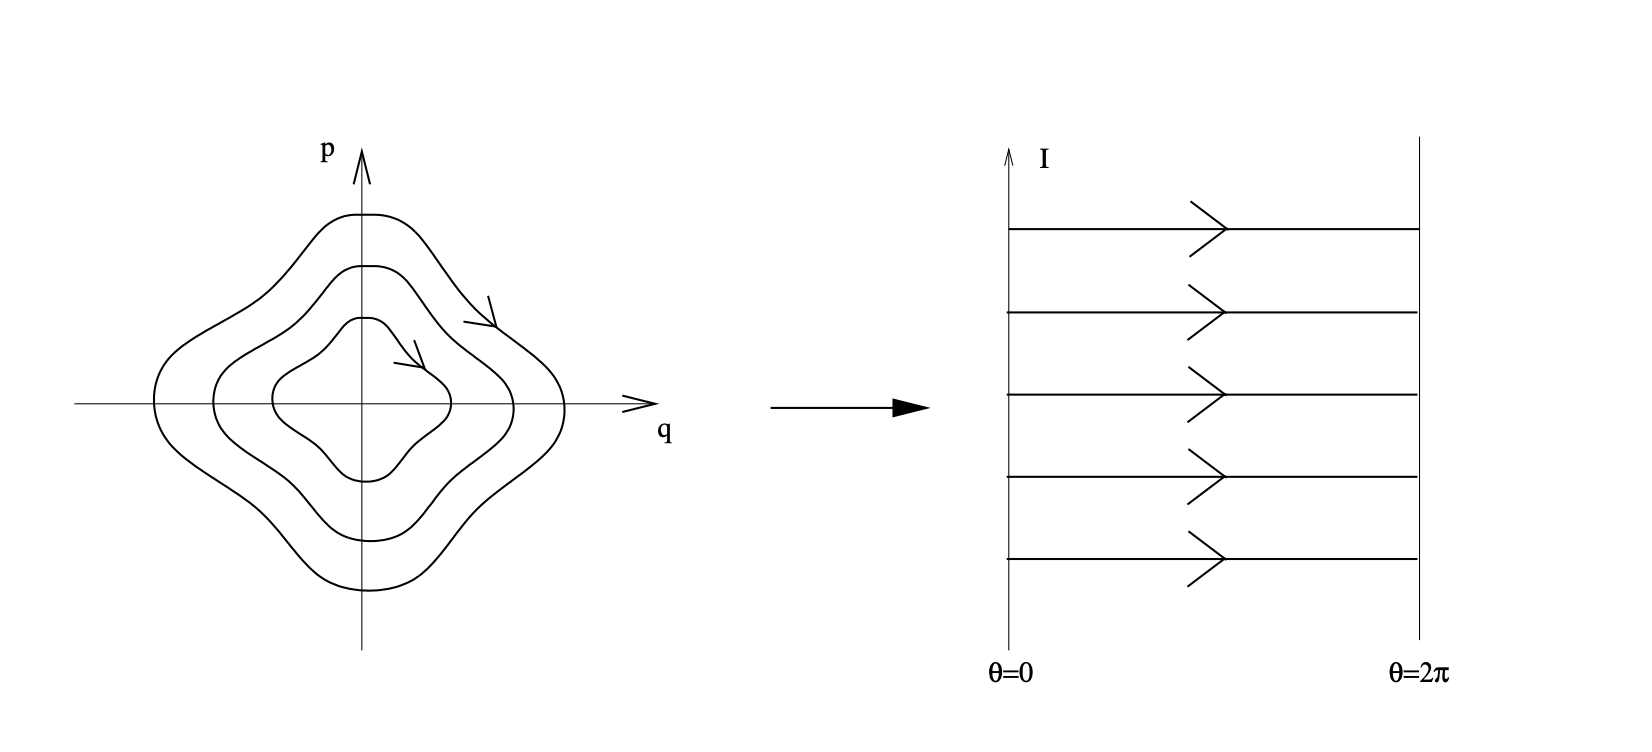
\includegraphics[width=0.95\textwidth]{figures/flow lines.png}
    \caption{transformation from $(q,p)$ to $(\theta,I)$ \cite{DavidTong}}
    \label{flow lines action}
\end{figure}


\begin{definition}
   Let $ H(q,p) $ be the Hamiltonian  for a one dimensional conserved mechanical system. Then the action variable $I$ is defined as
$$
I = \frac{1}{2\pi} \int_{H=E} p\,dq,
$$
where the integral is taken over the area enclosed by a periodic orbit in phase space, normalised by $2\pi$. The frequency associated with the orbit is then given by
$$\omega \defequal \dot{\theta} = \pd{H(\textbf{I})}{I}.$$
\end{definition}

A few important observations follow. First, the periodic orbit is uniquely determined by the energy $E$ since $H=E$, the action variable $I$ depends only on $E$ and is therefore conserved. Second, The transformation to action-angle variables is canonical; however, we will not explicitly prove this in this report and will instead assume it as given.

 The crucial statement in this construction was $H$ was conserved, turns out this enough for a one dimensional system to be integrable. However, if a system is integrable and there exists compact level set then we may be able to construct action-angle variables via the Liouville-Arnold theorem we shall now motivate this theorem in the following section.

\section{Symplectic Geometry }\label{Symplectic geometry sec} 

In this section, we provide a brief introduction to symplectic geometry, highlighting its role in Hamiltonian mechanics and its relevance to the Liouville-Arnold theorem. Proofs are omitted for conciseness, but references for further details can be found in \cite{arnol2013mathematical} and \cite{TMPB23/24}. This report is largely self-contained, assuming a background in Lagrangian mechanics and some familiarity with ordinary differential equations (ODEs). However, for this section, we assume prior knowledge of differential geometry, particularly from the differential geometry course \cite{DifferentialGeometry}.

Hamiltonian mechanics describes the evolution of a mechanical system in phase space, which, for a system with 
$n$ degrees of freedom, is a $2n$-dimensional manifold. The coordinates of this manifold consist of $n$ position variables and their conjugate momenta. The system's evolution is governed by a function on phase space known as the Hamiltonian.

To develop this framework, we first introduce key concepts from symplectic geometry, including Hamiltonian vector fields and their flows. Building on these foundations, we then present the Liouville-Arnold theorem, which formalises the notion of integrability in our context.  

\subsection{Symplectic Manifolds and Darboux’s Theorem}

\begin{definition}[Symplectic Vector space] A symplectic vector space is a pair ($V$,$\omega$), where $V$ is a $2n$-dimensional real vector space and symplectic structure $\omega \in \Lambda^{2}V$ is a skew-symmetric, non-degenerate bilinear form on $V$. Explicitly, $\omega: V \times V \rightarrow \R$ such that 
$$\omega(\textbf{u},\textbf{v}) = -\omega(\textbf{v},\textbf{u}) \ \forall \ \textbf{u} ,\textbf{v} \in V \ \ (\text{skew-symmetry}) $$
$$\omega(\textbf{u},\textbf{v}) = 0 \ \forall \ \textbf{u} \in V  \implies \textbf{v} = 0 \ (\text{non-degenerate}). $$
    
\end{definition}
\begin{remark}\label{symplectic vector space example}
    The symplectic structure may already be familiar. Recall the matrix \( \Omega \) from \autoref{symplectic}. Using this, we obtain the canonical example of a symplectic vector space,  $V=\R^{2n}$ and $\omega(\textbf{u},\textbf{v}) = \textbf{u}^{T}\Omega \textbf{v}$.
\end{remark}

\begin{definition}[Symplectic Manifold]
    A symplectic manifold is a pair $(M,\omega)$ where $M$ is a 2$n$-dimensional smooth manifold and $\omega \in \Omega^{2}(M)$ satisfying:
    $$ d \omega = 0 \ \ (\omega \ \text{is a closed  2-form})$$
    $$ \omega(X,Y) = 0 \ \forall X \ \in \mathfrak{X}(M) \implies Y = 0 \ (\text{non-degenerate})$$
\end{definition}

The two-form $\omega$ is called a symplectic form. Importantly, at each point $p\in M$, the tangent space $T_{p}M$ inherits structure of a symplectic vector space.

\begin{example}
Let $M = \mathbb{R}^{2n}$ with coordinates $(p_i,q_i)$ for $i \in \{1,\dots,n\}$ and
\[
\omega = \sum_{i=1}^{n} dp_i \wedge dq_i.
\]
Here $\omega$ is exact (since $\omega = d(p_i\, dq_i)$) and hence closed. In the coordinate basis $\{\frac{\partial}{\partial p_i},\frac{\partial}{\partial q_i}\}$ we have
\[
\omega\left(\frac{\partial}{\partial p_i},\frac{\partial}{\partial p_j}\right)=0 \ , \quad \omega\left(\frac{\partial}{\partial q_i},\frac{\partial}{\partial q_j}\right)=0 \ , \ 
\omega\left(\frac{\partial}{\partial p_i},\frac{\partial}{\partial q_j}\right)=\delta_{ij}.
\]
Thus, the matrix representation of $\omega$ is invertible at every point, making $\omega$ non-degenerate. The coordinate system $(p_i,q_i)$ is then said to be a {symplectic chart}.
\end{example}



\begin{definition}[Symplectic Chart]
A \emph{symplectic chart} on $(M,\omega)$ is a coordinate chart $(p_i,q_i)$, $i \in \{1,\dots,n\}$, on $M$ such that
$$
\omega = \sum_{i=1}^{n} dp_i \wedge dq_i.
$$
This is equivalent to the coordinate basis $\{\frac{\partial}{\partial p_i},\frac{\partial}{\partial q_i}\}$ being a symplectic basis.
\end{definition}
\noindent We now state one of the central result of symplectic geometry.

\begin{theorem}[Darboux]
Let $(M,\omega)$ be a symplectic manifold. Then every point $p\in M$ is contained in a symplectic chart.
\end{theorem}

\begin{remark}
 Darboux’s theorem implies that all symplectic manifolds are locally equivalent to a symplectic vector space. Moreover, one can show that all symplectic vector spaces correspond to the one from Remark \ref{symplectic vector space example}.
 \end{remark}
Before proceeding, we briefly discuss the significance of symplectic geometry in classical mechanics. Consider the following construction. Let $Q$ be the configuration space which is an $n$-dimensional smooth manifold with a chart $\phi(x) = (q_{i}(x))$ containing the point $x \in Q$. Then the cotangent bundle $T^{*}Q = \{(p_{x},x)| p_{x} \in T^{*}_{x}Q \ ,\ x \in Q \}$ is the phase space of the system and a $2n$-dimensional smooth manifold \footnote{This has been proved in the differential geometry course, see \cite{DifferentialGeometry}.} which has a chart $\Phi(p_{x},x) = (p_{i}(x),q_{i}(x))$, where $p_{i}$ are component functions of the 1-form $p_{x} = p_{i}(x)(dq_{i})_{x}$. 
\begin{theorem}
    $T^{*}Q$ has a symplectic form $\omega$ which in the above chart is
    $$ \omega = \sum_{i}dp_{i} \wedge dq_{i.}$$
\end{theorem}

\begin{remark}
   This provides a precise mathematical definition of phase space in a geometric context. For the purposes of this report, unless explicitly stated otherwise, we assume phase space to be diffeomorphic to \( \mathbb{R}^{2n} \), as our configuration spaces are taken to be \( \mathbb{R}^{n} \).
\end{remark}



\subsection{Hamiltonian Vector Fields and the Poisson Bracket}

We now derive Hamilton’s equations from a geometric perspective.

\begin{definition}[Hamiltonian Vector Field]
Let $X_{H}$ be a Hamiltonian vector field associated with the Hamiltonian function $H \in C^\infty(M)$. It is defined by $$
\iota_{X_H}\omega = -dH.
$$
In local symplectic coordinates $(p_i,q_i)$, along an integral curve $\dot{\gamma} = X_{H}(\gamma(t))$, this definition leads to Hamilton’s equations:
$$
\dot{q}_i = \frac{\partial H}{\partial p_i}, \quad \dot{p}_i = -\frac{\partial H}{\partial q_i}.
$$
\end{definition}

\begin{definition}[Poisson Bracket]
For functions $f,g\in C^\infty(M)$, we define the Poisson bracket as follows
$$
\pb{f}{g} := X_g(f) = -\omega(X_f,X_g).
$$
In a symplectic chart $(p_i,q_i)$ the Poisson bracket takes the familiar form from Definition \ref{poisson bracket}
$$
\pb{f}{g} = \sum_{i=1}^{n}\left(\frac{\partial f}{\partial q_i}\frac{\partial g}{\partial p_i} - \frac{\partial f}{\partial p_i}\frac{\partial g}{\partial q_i}\right).
$$
\end{definition}
We now introduce the notion of a Hamiltonian system and its constants of motion in a geometric framework.
\begin{definition}
    A Hamiltonian system $(M,\omega;H)$ is a symplectic manifold $(M,\omega)$ with a preferred function $H \in C^{\infty}(M)$ called the Hamiltonian. Motion, or `time-evolution', of a Hamiltonian system is defined by the Hamiltonian flow of $X_{H}$ (which is a Hamiltonian vector field.).
\end{definition}

\begin{definition}[Constant of Motion]
A constant of motion (or first integral) of a Hamiltonian system \( (M,\omega;H) \) is any function \( f \in C^{\infty}(M) \) that is invariant under the flow of \( X_H \). Thus, \( f \) is a constant of motion if and only if it commutes with \( H \) under the Poisson bracket:
\[
\{ f, H \} = 0.
\]
\end{definition}

\begin{theorem}
The Hamiltonian \( H \) is invariant under the flow of \( X_f \) if and only if \( f \in C^{\infty}(M) \) is a constant of motion.
\end{theorem}

\begin{proof}
Recall that 
\[
X_f(H) = \{ H, f \} = -\{ f, H \}.
\]
Therefore, \( X_f(H) = 0 \) if and only if \( \{ f, H \} = 0 \), as required.
\end{proof}




\subsection{Liouville Integrability and the Liouville–Arnold Theorem}

In Hamiltonian mechanics, a system is integrable in the Liouville sense if it satisfies the following conditions.

\begin{definition}\label{liouville}
A $2n$-dimensional Hamiltonian system $(M,\omega;H)$ is Liouville integrable if:
\begin{enumerate}
    \item There exist functions $
    f_1:= H, \, f_2, \dots, f_n \in C^\infty(M)$ that are in {involution}, i.e.
    $$
    \pb{f_{i}}{f_{j}} = 0,\quad \forall\, i,j=1,\dots,n.
    $$
    \item The functions $f_i$ are independent on the level sets
    $$
    M_c := \{ p \in M \mid f_i(p)=c_i,\; i=1,\dots,n \},
    $$
    that is, the $1$-forms $df_i$ are linearly independent on $M_c$.
\end{enumerate}
\end{definition}

\begin{remark}
 It is known (see \cite{arnol2013mathematical}) that a  $2n$-dimensional symplectic manifold can admit at most $n$ independent functions in involution.
\end{remark}

The Liouville–Arnold theorem describes the structure of phase space for Liouville-integrable systems.

\begin{theorem}[Liouville–Arnold Theorem]\label{Liouville-Arnold}
Let $(M,\omega;H)$ be a $2n$-dimensional Hamiltonian system that is Liouville integrable. Then:
\begin{enumerate}
    \item The common level set 
    $$
    M_c := \{ p \in M \mid f_i(p) = c_i ,\text{ for } i = 1,\dots,n \},
    $$
    is a smooth $n$-dimensional submanifold that is invariant under the flow of $X_H$.
    \item If $M_c$ is compact and connected, then it is diffeomorphic to an $n$-torus
    $$
    T^n = \{ (\theta_1,\dots,\theta_n) \,\, \text{mod}\,\, 2\pi \}.
    $$
    \item The flow of $X_H$ on a compact $M_c\cong T^n$ takes the form
    $$
    \dot{\theta}_i = \omega_i(\mathbf{c}),
    $$
    where $\omega_i$ depend on the constant values $\mathbf{c}$.
    \item In a neighbourhood of $M_c\cong T^n$, there exist canonical {action–angle coordinates} $(I_i,\theta_i)$ such that the actions $I_i=I_i(\mathbf{c})$ are constants of motion.
\end{enumerate}
\end{theorem}
\begin{remark}
For $n=1$, the $1$-torus is a circle ($S^1$). For $n=2$, $T^2$ is topologically equivalent to a torus (or $S^1\times S^1$).  
\end{remark}
Geometrically, this result reveals that the phase space of an integrable system is foliated by an invariant tori, where each torus represents a compact, regular orbit on which the dynamics are quasi-periodic. This rich geometric structure highlights how integrability partitions the phase space into regions of regular motion. Having established the notion of integrability and the existence of action-angle variables via \autoref{Liouville-Arnold}, we conclude this chapter with their general definition. In the following chapters, we will explore examples of how to determine these variables using the Hamilton–Jacobi equation.

\begin{definition} \label{Action-angle-generalised}
    Let $\gamma_{i}$   denote a basis of one dimensional cycles on the torus $M_{\textbf{c}} \cong T^{n}$, where $i \in \{1,\cdots,n\}$. The action variables are defined by
    \begin{equation}
        I_{i}(\textbf{c}) = \cfrac{1}{2\pi} \int_{\gamma_{i}} \sum_{j}p_{j}dq_{j}.
    \end{equation}
\end{definition}
\begin{remark}
  A few remarks: First, when comparing with the $n=1$ case from the previous section we see that the level set $M_{c}$ is just the locus $H(p,q) = E$ and thus must be diffeomorphic to a circle. Therefore the two definitions are compatible. Second, notice that proving this change of variables is canonical amounts to proving that $(I_{i}$,$\theta_{i})$ are symplectic coordinates as this yields Hamilton's equation. While we do not prove it in this report, the proof is available in \cite{arnol2013mathematical}.
\end{remark}




 


\chapter{Kepler's Problem}\label{Kepler chapter}

\section{Introduction}

This chapter examines the Kepler problem in $\R^{3}$. The Kepler problem is a special case of the two-body problem in classical mechanics, where two bodies interact through a central force that follows an inverse-square law. We will structure this chapter as follows: First, we set up the problem, then identify the constants of motion, and demonstrate that the system satisfies the integrability criteria established in Definition \ref{liouville}. Next, we analyse the explicit solution of the problem before finally using  \autoref{Liouville-Arnold} to construct action-angle variables. 

We begin by constructing the Lagrangian for the problem. Consider the position vector in $\R^{3}$:
\[
    \textbf{X} = 
    \begin{bmatrix}
           x \\
           y \\
           z
         \end{bmatrix} 
         = \begin{bmatrix}
           r\sin{\theta} \cos{\varphi} \\
           r\sin{\theta} \sin{\varphi} \\
           r\cos{\theta}
         \end{bmatrix}.
\]
This leads to a kinetic and potential term:
\begin{align*}
T = \frac{M}{2} \langle {\dot{\textbf{X}}},{\dot{\textbf{X}}} \rangle &= \frac{M}{2} (\dot{r}^2 + r^2 \dot{\theta}^2 + r^2 \sin^2{\theta}\, \dot{\varphi}^2), \\ V &= \frac{-GMm}{r},
\end{align*}
where \(\langle \cdot , \cdot \rangle\) denotes the standard Euclidean inner product in \(\mathbb{R}^3\). The mass  of the fixed centre and of the moving body are $m$, $M$ respectively, and $G$ is the gravitational constant. For convenience we shall set the mass of the moving body to unity $M= 1$ and define the constant $\mu$ as, $\mu := Gm$.   


Since the problem has a natural spherical symmetry, spherical coordinates provide the most convenient representation. The Lagrangian of the system now reads:
\begin{equation}\label{2.1}
\mathcal{L}(q,\dot{q},t) = T-V = \frac{1}{2} (\dot{r}^2 + r^2 \dot{\theta}^2 + r^2 \sin^2{\theta}\, \dot{\varphi}^2) + \frac{\mu }{r}.
\end{equation}
This leads to the following second-order ODEs via the Euler-Lagrange equations:
\begin{itemize}
    \item For \( \varphi \):
    \begin{equation}\label{2.2}
      \frac{d}{dt} \left[  r^2 \sin^2{\theta} \dot{\varphi} \right] = 0.
    \end{equation}
      
    
    \item For \( \theta \):
    \begin{equation}\label{2.3}
        \frac{d}{dt} \left[ r^2 \dot{\theta} \right] = r^2 \sin{\theta} \cos{\theta} \dot{\varphi}^2.
    \end{equation}
    \item For \( r \):
    \begin{equation}\label{2.4}
        \frac{d}{dt} \left[ \dot{r} \right] = r \dot{\theta}^2 + r \sin^2{\theta} \dot{\varphi}^2 - \frac{\mu}{r^2}.
    \end{equation}
\end{itemize}

\section{Constants of motion}\label{constant of motion kepler}
We begin by identifying the constants of motion, starting with the conservation of the conjugate momentum associated with $\varphi$, denoted as $p_{\varphi}$. By noting that $p_{\varphi}$ is a constant and using \autoref{2.2}, we get
\begin{equation}\label{2.5}
    \dot{\varphi} = \frac{p_{\varphi}}{r^{2}\sin^{2}{\theta}}, 
\end{equation}
\noindent which allows us to rewrite  \autoref{2.3} as

$$ \frac{d}{dt} \left[ r^2 \dot{\theta} \right] = \cfrac{\cos{\theta}  p_{\varphi}^{2}}{r^{2}\sin^{3}{\theta}}, $$
in which upon multiplying both sides by $2r^{2} \dot{\theta}$ and rearranging terms, we find another conserved quantity

\begin{equation}\label{2.6} J^{2} = (r^{2}\dot{\theta})^{2} + \cfrac{p_{\varphi}^{2}}{\sin^{2}{\theta}} \ .
\end{equation}
The constant $J^{2}$ corresponds to the conservation of the total angular momentum squared, implying confinement of the body to a plane. The third conserved quantity is the total energy of the system which may be derived by using \autoref{2.5} and  \autoref{2.6},  simplifying  \autoref{2.4} as
\begin{equation}\label{2.8}
 \cfrac{\dot{r}^{2}}{2}  + \cfrac{J^{2}}{2r^{2}}  - \cfrac{\mu}{r} = -\alpha^{2}.
    \end{equation}
 This is expected since the Hamiltonian is time independent \footnote{As we shall see in the next section.} and here we have chosen the sign of the constant $\alpha^2$ so that the orbit remains bounded. Since we have identified three conserved quantities, we proceed to find the Hamiltonian and verify that the Kepler problem in $\mathbb{R}^{3}$ is integrable in the Liouville sense. 
\subsection{Hamiltonian Formulation and Integrability}
To demonstrate the integrability of the system, we first determine the constants of motion in coordinates $(q_{i},p_{i})$. By Definition \ref{Hamiltonian} the conjugate momenta associated to $(r,\theta, \varphi)$ are given by

\begin{equation} \label{2.25}
    p_{r} = \frac{\partial L}{\partial \dot{r}} = \dot{r},
\end{equation}
\begin{equation} \label{2.26}
    p_{\theta} = \frac{\partial L}{\partial \dot{\theta}} = r^{2} \dot{\theta},
\end{equation}
\begin{equation} \label{2.27}
    p_{\varphi} = \frac{\partial L}{\partial \dot{\varphi}} = r^{2} \sin^{2}{\theta} \dot{\varphi}.
\end{equation}
Since $M = 1$, we obtain the Hamiltonian by Definition \ref{Hamiltonian}, as follows

$$ H = \sum_{i}p_{i}\dot{q_{i}} - \mathcal{L}=\cfrac{1}{2} \left( p_{r}^{2}+\cfrac{p_{\theta}^{2}}{r^{2}}+\cfrac{p_{\varphi}^{2}}{r^{2}\sin^{2}{\theta}} \right) -\cfrac{\mu}{r}.$$
The Hamiltonian is a conserved quantity so we take the level set as $H=-\alpha^{2}$ as in the above section \ref{constant of motion kepler}. The remaining constant of motion, $J^{2}$ is explicitly given by
\begin{equation}\label{2.28}
    J^{2} = p_{\theta}^{2} + \cfrac{p_{\varphi}^{2}}{\sin^{2}{\theta}} \ .
\end{equation} 
To ensure consistency, we define a function $f_{J}$ as $f_{J} = p_{\theta}^{2}+\frac{p_{\varphi}^{2}}{\sin^{2}{\theta}}-J^{2}$, the level set is then given by $f_{J} = 0$.
To check for involution, we recall the Poisson bracket relation, given by Proposition \ref{pbrel}
$$ \td{f}{t} = \pd{f}{t} + \{f,H\}.$$
From the definition of constants of motion, we get
$$ \{f_{J},H\} = \td{f_{J}}{t} = 0,$$
$$ \{H,H\} = \td{H}{t} = 0,$$
$$ \{p_{\varphi},H\} = \td{p_{\varphi}}{t} = 0,$$
thus the only thing remaining to check is $\{f_{J},p_{\varphi}\}$. We have
$$ \{f_{J},p_{\varphi}\} = \left\{ p_{\theta}^{2} + \cfrac{p_{\varphi}^{2} }{\sin^{2}{\theta}}-J^{2} , p_{\varphi} \right\} $$
hence by bi-linearity of the Poisson bracket, we obtain
$$  = \left\{ p_{\theta}^{2} , p_{\varphi} \right\}  + \left\{  \cfrac{p_{\varphi}^{2}}{\sin^{2}{\theta}} , p_{\varphi} \right\}-\pb{J^{2}}{p_{\varphi}} = 0.$$
The first term is zero because of the identity from \autoref{useful id} and the other two terms  evaluate to zero. Thus, the quantities $H$, $f_{J}$, and $p_{\varphi}$ are in involution. Next, we verify the independence of $H, f_{J}, p_{\varphi}$ on level sets by considering the following expression


$$ H = -\alpha^{2} \ , \ p_{\varphi} = C , \ f_{J} = 0,$$
where $J,\alpha ,C \in \R$. Now consider the differential of these functions on the above level sets
\[
dH = \left( -\frac{p_\theta^2}{2r^3} - \frac{p_\varphi^2}{2r^3 \sin^2\theta} + \frac{\mu}{r^2} \right) dr 
- \frac{p_\varphi^2 \cos\theta}{r^2 \sin^3\theta} d\theta 
+ p_r dp_r 
+ \frac{p_\theta}{r^2} dp_\theta 
+ \frac{p_\varphi}{r^2 \sin^2\theta} dp_\varphi,
\]
$$dp_{\varphi} = dp_{\varphi},$$
 $$ f_{J}= d\left(\ p_{\theta}^{2} + \cfrac{p_{\varphi}^{2}}{\sin^{2}{\theta}}-J^{2}\right)= -\frac{2 p_{\varphi}^{2} \cos{\theta}}{\sin^{3}{\theta}} d\theta 
+ 2 p_{\theta} dp_{\theta} 
+ \frac{2 p_{\varphi}}{\sin^{2}{\theta}} dp_{\varphi} .$$ 
To prove linear independence consider the following linear combination
$$ adH + bdf_{J} + cdp_{\varphi} = 0$$
where $a,b,c \in \R$. Examining the coefficient of $dr$ and noting we're looking at it on the level set we get
$$\frac{a}{r^{2}}\left(\mu r - \frac{J^{2}}{2}\right) = 0.$$
However, we notice this has to be true for arbitrary $r$ on the level set for fixed $J \in \R$ and because the 1-forms $dq_{i}$'s and $dp_{i}$'s forms a basis at the cotangent space at the level set, we conclude that $a =0$. Now considering the coefficient of $dp_{\varphi}$ which gives
$$ b\frac{2p_{\varphi}}{\sin^{2}{\theta}} + c =0.$$
Since this holds for arbitrary $\theta$ in the level set and assuming $\theta$ is not degenerate we conclude $b = 0$.  This means $a=b=c=0$ which implies the constants of motion are linearly independent on the level sets hence the system is Liouville integrable by Definition \ref{liouville}.

\section{Solving for Trajectories}
Now that we have shown the system is integrable, we proceed to find explicit solutions for the trajectories. We begin by introducing a new independent variable $f$, which satisfies

\begin{equation}\label{2.9}
    J\cfrac{d}{df} = r^2\cfrac{d}{dt}.
\end{equation}
Substituting this into \autoref{2.5}, \autoref{2.6}, and \autoref{2.8}, we obtain

\begin{subequations}
 \begin{equation}\label{2.10}
    \sin^{2}{\theta}\left(\cfrac{d\theta}{df} \right)^{2} = \left(1- \cfrac{p_{\varphi}^{2}}{J^{2}} \right)-\cos^{2}{\theta},
\end{equation}  
 \begin{equation}\label{2.11}
    \left( \cfrac{dr}{df} \right)^{2} = -r^{2} \left[ 1 - \cfrac{2 \mu r}{J^{2}} + \cfrac{2\alpha^{2}r^{2}}{J^{2}}\right],
\end{equation}
\begin{equation}\label{3.13c}
  \td{\varphi}{f} = \cfrac{\frac{p_{\varphi}}{J}}{\sin^{2}{\theta}}.  
\end{equation}
\end{subequations}

\begin{remark}[Notation]
For convenience, we denote $\cfrac{d}{df}$ as $^{\prime}$ i.e., $\td{R}{f}$ will be written as $R^{\prime}$
\end{remark}
We now solve for the trajectory of $r$ in terms of the angle parameter $f$. Substituting 
$$ u = \cfrac{1}{r}, r = \cfrac{1}{u}, \ \text{where} \ r^{\prime} = -\cfrac{u^{\prime}}{u^{2}},$$ 
we get
$$ {u^{\prime}}^{2} = -\left[ u^{2} - \cfrac{2 u\mu }{J^{2}} + \cfrac{2\alpha^{2}}{J^{2}}\right]. $$
Completing the square on the right-hand side and defining
$$ u - \cfrac{\mu}{J^{2}}= \sqrt{\cfrac{\mu^{2}}{J^{4}} - \cfrac{2\alpha^{2}}{J^{2}}} w, $$
we obtain
$$ {w^{\prime}}^{2} = 1 - w^{2}, $$
giving the solution
$$ w = \cos{(f+\omega_{0})}. $$
Here, $\omega_{0}$ is an integration constant. Returning to $r$ we get

\begin{equation} \label{2.12}
    r = \cfrac{\cfrac{J^{2}}{\mu}}{1 + \sqrt{1-\cfrac{2J^{2}\alpha^{2}}{\mu^{2}}} \cos{(f+\omega_{0})}}.
\end{equation}

\begin{remark}
The quantity $ \sqrt{1-\frac{2J^{2}\alpha^{2}}{\mu^{2}}}  $ is usually denoted as $e$, the eccentricity of the orbit \cite{o2008integrable}. In particular, $e \lesseqgtr 1$ corresponds to negative/positive energy solutions, representing elliptic/hyperbolic orbits. If $e = 0$, the orbit is circular.
\end{remark}
Returning to solving \autoref{2.10} for $\theta$, we introduce the substitution
$$ \cos{\theta} = \sqrt{1- \cfrac{p_{\varphi}^{2}}{J^{2}}} S, $$
which leads to
$$ {S^{\prime}}^{2} = 1 - S^{2}, $$
giving the solution
$$ S = \sin{(f+\omega_{1})}. $$
Again, $\omega_{1}$ is an integration constant, and we obtain

\begin{equation}
    \cos{\theta}=\sqrt{1- \cfrac{p_{\varphi}^{2}}{J^{2}}} \sin{(f+\omega_{1})}.
\end{equation}

Finally, we solve \autoref{3.13c} for $\varphi$. Substituting the solution for $\cos{\theta}$ and simplifying, we get
$$  \varphi^{\prime} = \cfrac{\cfrac{p_{\varphi}}{J} \sec^{2}{(f+\omega_{1})}}{1 + \left(  \cfrac{p_{\varphi}}{J} \right)^{2} \tan^{2}{(f+\omega_{1})}}. $$
Defining $\tan{\phi} = \cfrac{p_{\varphi}}{J}\tan{(f+\omega_{1})}$, and differentiating with respect to $f$, we get
$$ \sec^{2}{(\phi)} \phi^{\prime} = \cfrac{p_{\varphi}}{J} \sec^{2}{(f+\omega_1)}, $$
where
$$ \sec^{2}{\phi} = 1+\left( \cfrac{p_{\varphi}}{J} \right)^{2}\tan^{2}{(f+\omega_1)}. $$
This implies $\phi^{\prime} = \varphi^{\prime}$, leading to

$$ \phi = \varphi + \varphi_{0}, $$
where $\varphi_{0}$ is an integration constant. This results in the equation for $\varphi$

\begin{equation}\label{2.15}
    \tan{(\varphi+\varphi_{0})} = \cfrac{p_{\varphi}}{J}\tan{(f+\omega_{1})},
\end{equation}

which completes the solution for the trajectories in terms of the variable $f$, which is often called the true anomaly \cite{o2008integrable}. For completeness, we solve for the time-angle relationship in Appendix \ref{appendix1}.


\section{Action-Angle Variables for Kepler}\label{Kepler Action angle}
In this section, we examine the implication of the Liouville-Arnold \autoref{Liouville-Arnold} and explicitly construct action-angle variables for this problem. We start by once again recalling the conserved quantities for the system:
\begin{align*}
    -\alpha^{2} &= \cfrac{1}{2} \left( p_{r}^{2}+\cfrac{p_{\theta}^{2}}{r^{2}}+\cfrac{p_{\varphi}^{2}}{r^{2}\sin^{2}{\theta}} \right) -\cfrac{\mu}{r},
    \\
    J^{2} &= p_{\theta}^{2} + \cfrac{p_{\varphi}^{2}}{\sin^{2}{\theta}},
    \\
     C &= p_{\varphi} .
\end{align*}
 Since the Hamiltonian is time-independent, we can apply Proposition \ref{Time independent HJ} to obtain
$$ H\left(q_{i},\pd{W}{q_{i}},t \right)  = -\alpha^{2} \   ; \ \ p_{i} = \pd{W}{q_{i}}.\ $$
We note that the sign is 
$-\alpha^{2}$ is to ensure bounded orbits. Additionally, one can show that this choice is necessary for obtaining compact level sets. Substituting the ansatz
$$W = W_{r}+W_{\theta}+W_{\varphi},$$
into the Hamilton-Jacobi equation and rearranging we obtain
$$ -2\alpha^{2}r^{2}\sin^{2}{\theta} + 2 \mu r\sin^{2}{\theta} - \left(\pd{W_{r}}{r}\right)^{2}r^{2}\sin^{2}{\theta} - \left( \pd{W_{\theta}}{\theta} \right)^{2}\sin^{2}{\theta} = \left( \pd{W_{\varphi}}{\varphi} \right)^{2}.$$
 Separating variables we arrive at 
 \begin{align}
     \pd{W_{\varphi}}{\varphi} &= C,
     \\
     \pd{W_{\theta}}{\theta} &= \sqrt{J^{2}-\cfrac{p_{\varphi}^{2}}{\sin^{2}{\theta}}},
     \\
      \pd{W_{r}}{r} &= \cfrac{\sqrt{-2\alpha^{2}r^{2}+2\mu r - J^{2}}}{r} .
 \end{align}
 %$$ -2\alpha^{2}r^{2}\sin^{2}{\theta} + 2 \mu r\sin^{2}{\theta} - \left(\pd{W_{r}}{r} \right)^{2}r^{2}\sin^{2}{\theta} - \left( \pd{W_{\theta}}{\theta}\right)^{2}\sin^{2}{\theta} = C^{2} $$
 %$$ \implies -2\alpha^{2}r^{2} + 2\mu r - \left( \pd{W_{r}}{r} \right)^{2}r^{2} =  \left( \pd{W_{\theta}}{\theta} \right)^{2} + \cfrac{C^{2}}{\sin^{2}{\theta}}  \defequal J^{2} $$
 Finally recalling the action-angle coordinate are given by Definition \ref{Action-angle-generalised}, we obtain
 \begin{align}
      I_{\varphi} &= \cfrac{1}{2\pi} \int_{\gamma_{\varphi}} \ C \ d \varphi ,
      \\
       I_{\theta} &= \cfrac{1}{2 \pi} \int_{\gamma_{\theta}} \ \sqrt{J^{2}-\cfrac{p_{\varphi}^{2}}{\sin^{2}{\theta}}} \ d \theta ,\label{theta int}
      \\
        I_{r} &= \cfrac{1}{2 \pi} \int_{\gamma_{r}} \ \cfrac{\sqrt{-2\alpha^{2}r^{2}+2\mu r - J^{2}}}{r}  \ d r.
 \end{align}
 
 Where the limits of the integrals are determined by closed curves in phase space.
Since the Hamiltonian does not depend explicitly on $\varphi$, the coordinate is cyclic, and we obtain
 $$ I_{\varphi} = p_{\varphi}.$$
 \begin{figure}[ht!]
    \centering
    % First image: pr vs r
    \begin{subfigure}{0.85\textwidth} % Adjust width as needed
        \centering
        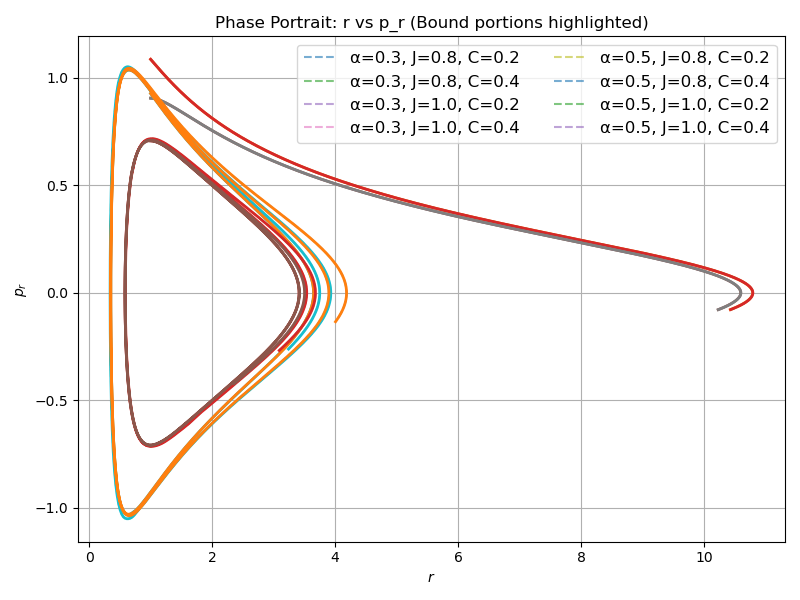
\includegraphics[width=\linewidth]{figures/p_r plot.png}
        \caption{Plot of \( p_r \) vs \( r \)}
        \label{fig:pr_vs_r}
    \end{subfigure}
    \hfill
    % Second image: ptheta vs theta
    \begin{subfigure}{0.85\textwidth} % Adjust width as needed
        \centering
        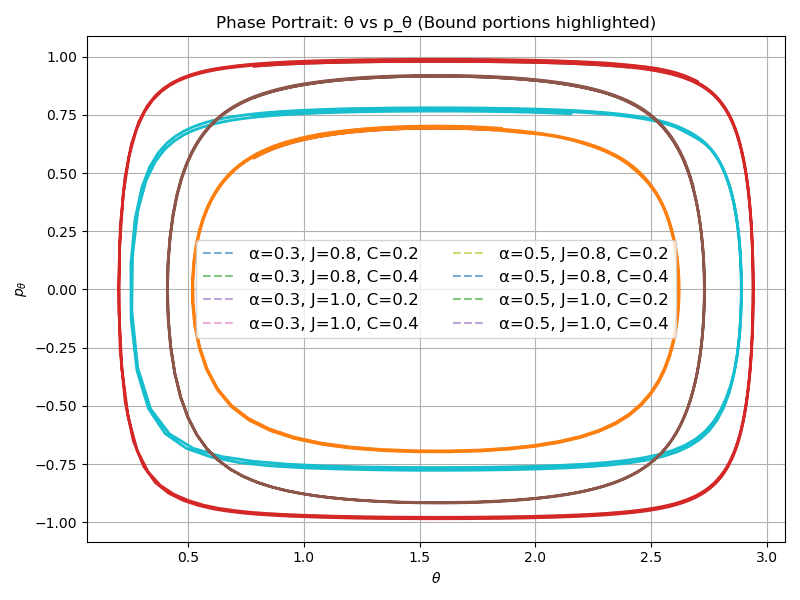
\includegraphics[width=\linewidth]{figures/p_theta plot.png}
        \caption{Plot of \( p_{\theta} \) vs \( \theta \)}
        \label{fig:ptheta_vs_theta}
    \end{subfigure}
    \caption{Phase portraits illustrating the motion in $r-p_{r}$ and $\theta-p_{\theta}$ phase space. These were generated numerically for different values of $J,C,\alpha$. }
    \label{fig:side_by_side}
\end{figure}
To evaluate $I_{\theta}$, we identify the integration limits as the closed curve spanning from $-\theta^{*}$ to $+\theta^{*}$ in phase space. The shape of this curve is determined by the condition $p_{\theta}|_{\theta = \theta^{*}} = 0$ (see figure  \ref{fig:ptheta_vs_theta}), ensuring  the local maxima/minima of the motion with respect to $t$. Since the motion is symmetric, we compute the integral from $\frac{\pi}{2}$ to $\theta^{*}$ and multiply by 4. Introducing
$\frac{p_{\varphi}}{J} = \cos{l}$ (this is known as the polar angle \cite{goldstein2002classical} and is a unit less parameter)  we get a convenient relationship of $\theta^{*} = \frac{\pi}{2} -l $. 
\begin{remark}
   A quick remark here, $\frac{p_{\varphi}}{J} = \cos{l}$ is a valid substitution as for $I_{\theta}$ to be a valid closed curve $\frac{p_{\varphi}}{J} \leq 1$.
\end{remark}
\noindent Thus, integral \ref{theta int} may be rewritten as
$$I_{\theta} = \cfrac{2J}{\pi} \int_{\frac{\pi}{2}}^{\theta^{*}}  \csc{\theta} \sqrt{\sin^{2}{\theta} - \cos^{2}{l}} \ d \theta  = \cfrac{2J}{\pi} \int_{\frac{\pi}{2}}^{\theta^{*}}  \csc{\theta} \sqrt{\sin^{2}{l} - \cos^{2}{\theta}} \ d \theta , $$
now using the substitution
$$ \cos{\theta} = \sin{l}\sin{\Phi}$$
gives
$$ I_{\theta} = \cfrac{2J\sin^{2}{l}}{\pi} \int_{0}^{\frac{\pi}{2}} \cfrac{\cos^{2}{\Phi}}{1-\sin^{2}{l}\sin^{2}{\Phi}} \ d \Phi. $$
We make one more substitution
$$ u = \tan{\Phi},$$
to get
$$I_{\theta} = \cfrac{2J\sin^{2}{l}}{\pi} \int_{0}^{\infty} \cfrac{1}{(1+u^{2})(1+u^{2}\cos^{2}{l})} \ du.$$
Which can be simplified via partial fractions and is a known integral that evaluates to
\begin{equation}
    I_{\theta} = J \left(1-\frac{p_{\varphi}}{J} \right) = J - p_{\varphi}.
\end{equation}
We now evaluate the final integral for $I_{r}$ which was given by
$$ I_{r} = \cfrac{1}{2 \pi} \int_{\gamma_{r}} \ d r \ \cfrac{\sqrt{-2\alpha^{2}r^{2}+\mu r - (I_{\theta}+I_{\varphi})^{2}}}{r} .$$
The limits of integration for $I_{r}$ are determined by the points where the expression under the square root vanishes, corresponding to the turning points of the radial motion (where $p_{r}=\dot{r} = 0$). Thus let $r_{+}$ and $r_{-}$ be the roots for the quadratic above, the closed counter then goes from $r_{-}$ to $r_{+}$ and then back to $r_{-}$ thus the integral may be written as 2 times the integral from $r_{-}$ to $r_{+}$,  i.e.
$$ I_{r} = \cfrac{1}{\pi} \int_{r_{-}}^{r_{+}} \cfrac{\sqrt{-2\alpha^{2}r^{2}+2 \mu r -(I_{\theta}+I_{\varphi})^{2}}}{r} \ dr.$$
\begin{remark}
    Note that the quadratic must have real roots; otherwise, no closed curve can exist. As seen in Figure \ref{fig:pr_vs_r}, for certain values of $J,\alpha,C \in \R$, not all trajectories in phase space correspond to closed orbits.
\end{remark}
\begin{figure}[htbp]
    \centering
    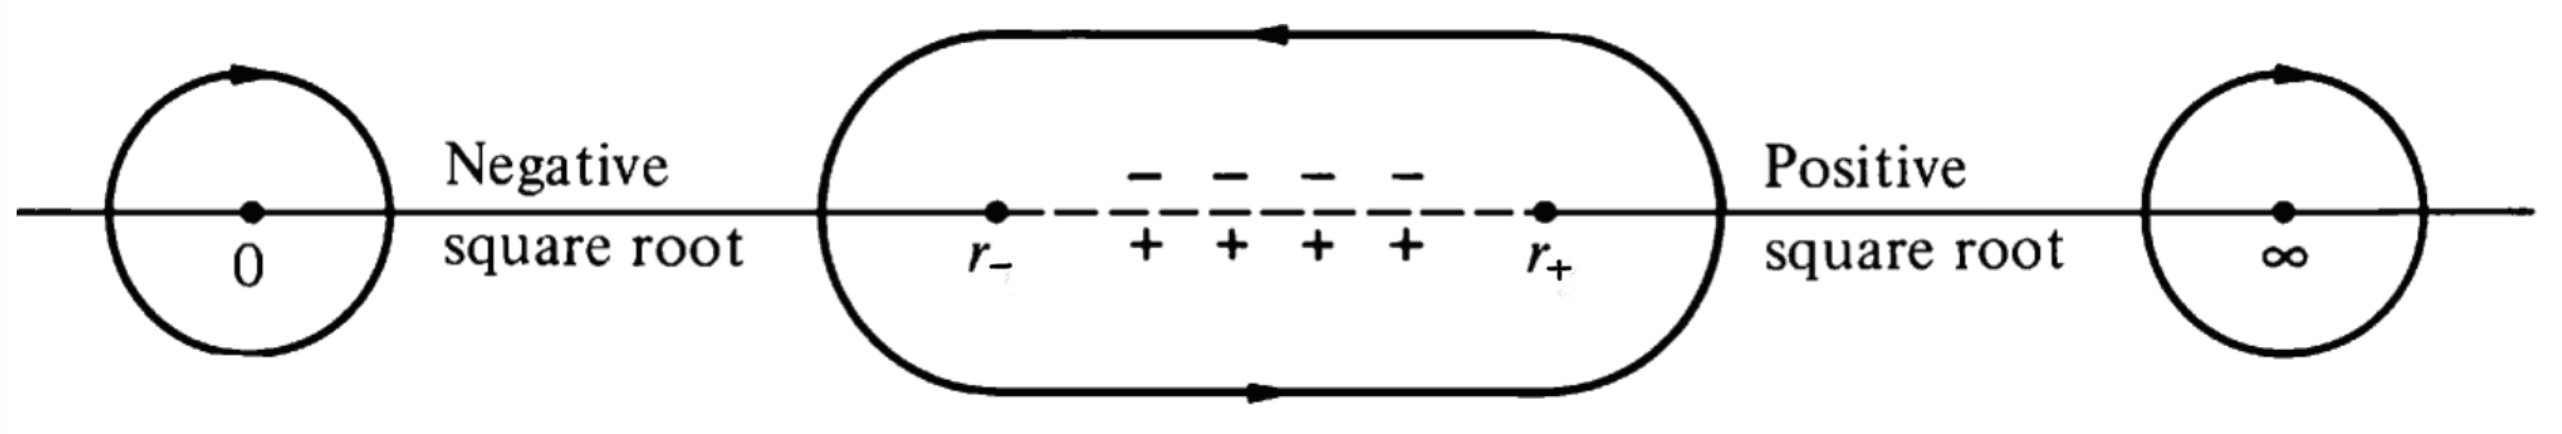
\includegraphics[width=0.95\textwidth]{figures/poles2.png}
    \caption{Complex plane r via in the neighbourhood of the real axis \cite{goldstein2002classical}}
    \label{Complex plane r}
\end{figure}
This integral can be evaluated via the use complex contour integration technique, identifying branch points at $r_{\pm}$ and enclosing the branch cut from $r_{-}$ to $r_{+}$ with a contour in the complex plane (as seen in \ref{Complex plane r}). We split the contour into four parts, where two of them cancel. The remaining two pick up a phase contribution from the branch cut, leading to an integral that is twice the real integral. Although we cannot directly apply the residue theorem to the given contour, we can instead consider its complement, which encloses the rest of the complex plane in the clockwise direction. This contour is analytic everywhere except at the poles at $r=0$ \& $r \rightarrow \infty$, allowing us to apply the residue theorem.
$$ 2I_{r} = \cfrac{2\pi i}{\pi} \left[ \text{Res}(I_{r},0) + \text{Res}(I_{r}, r\rightarrow \infty)\right].$$
  Using the residue formula for poles, at $r=0$ we get
$$ \text{Res}(I_{r},0) = \frac{1}{(1-1)!}\lim_{r\rightarrow 0} \cfrac{d^{0}}{dr^{0}} \left( {\cfrac{r\sqrt{-2\alpha^{2}r^{2}+2 \mu r -(I_{\theta}+I_{\varphi})^{2}}}{r}} \right)$$
$$ = i(I_{\theta} + I_{\varphi})$$
now at $r \rightarrow \infty$,
We first start by changing variables of the integral by setting $r = \frac{1}{z}$ and then evaluate the residue at $z = 0$,
$$ \text{Res}(I_{r},r \rightarrow \infty) = \frac{1}{(2-1)!}\lim_{z\rightarrow 0} \cfrac{d}{dz} \left( z^{2} \frac{-1}{z^{2}} \sqrt{-2\alpha^{2}+2\mu z -(I_{\theta}+I_{\varphi})^{2}z^{2}}  \right)$$
$$ = \cfrac{-\mu}{\sqrt{-2\alpha^{2}}}.$$
Putting it all together we get
$$  I_{r} = -(I_{\theta}+I_{\varphi}) -\frac{\mu i}{\sqrt{-2\alpha^{2}}} $$
$$ -\alpha^{2} = -\cfrac{\mu^{2}}{2(I_{r}+I_{\theta}+I_{\varphi})^{2}}.$$
Since the Hamiltonian is conserved and we define it such that $H = -\alpha^{2}$, thus in action-angle coordinates it is given by
\begin{equation}
    H = -\cfrac{\mu^{2}}{2(I_{r}+I_{\theta}+I_{\varphi})^{2}}.
\end{equation}
Now, considering the angular frequencies via \autoref{Liouville-Arnold}, we have  
\[
\omega_{i} = \dot{\theta_{i}},
\]  
which shows that the frequencies \(\omega_{i}\) are degenerate, as  
\[
\dot{\theta_r} = \dot{\theta_\theta} = \dot{\theta_\varphi} = \frac{\mu^2}{4(I_r + I_\theta + I_\varphi)^3}.
\]  
This degeneracy implies that the frequencies \(\omega_{i}\) are commensurate, meaning their ratios are rational. As a consequence, the trajectory in phase space is periodic, and the motion repeats after a finite time. Since a closed trajectory in phase space means that both position and velocity return to their initial values, the orbit in configuration space must also be closed.  

Thus, in the Kepler problem, bound orbits do not precess but remain elliptical. This is expected, as the solution to the orbital trajectories for \( e \leq 1 \) corresponds to an ellipse or a circle. In contrast, for more general gravitational systems, frequency degeneracies are broken, leading to precessing orbits, as we shall see in the following chapter.  







\chapter{Euler Problem Planar Case}

\section{Introduction}
The Planar Euler problem, also known as the two fixed centre problem, describes a system where three bodies interact in a plane. Two fixed masses are symmetrically situated  on the $z$ axis (at $z= \pm b$) where they induce a gravitational field on the free body $P$ (for simplicity, we assume $P$ is a point mass). We shall structure our discussion of this chapter in a similar fashion to \autoref{Kepler chapter}. Starting by addressing the potential and the choice of coordinates.
\begin{figure}[htbp]
    \centering
    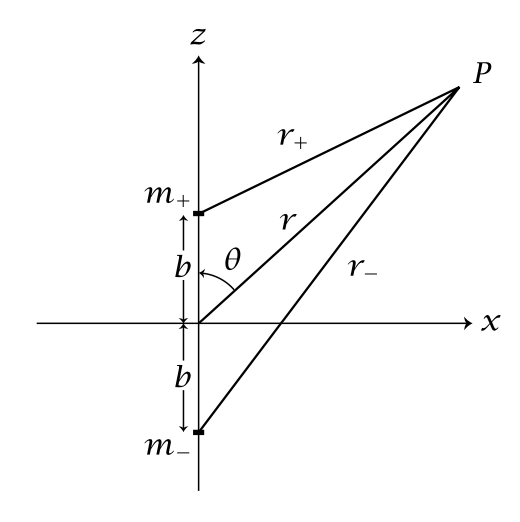
\includegraphics[width=0.55\textwidth]{figures/Euler problem I.png}
    \caption{Set up of the two fixed centre problem \cite{o2008integrable}}
    \label{fig:Euler problem I}
\end{figure}
The gravitational potential per unit mass at P is given by
\begin{equation} \label{3.1}
  V = G\left( \cfrac{m_{+}}{r_{+}} + \cfrac{m_{-}}{r_{-}}\right).  
\end{equation} 
Here, $G$ is the gravitational constant and the potential is given in terms of polar coordinates ($r,\theta$), where $\theta$ is measured from positive $z$ axis  (as indicated in Figure \ref{fig:Euler problem I}), the distances $r_{+}$ and $r_{-}$ are given by:
\begin{subequations}
    \begin{equation}\label{3.2a}
        r_{+}^{2} = r^{2} + b^{2} - 2br\cos{\theta} ,
    \end{equation}
    \begin{equation}\label{3.2b}
        r_{-}^{2}=r^{2}+b^{2}+2br\cos{\theta}.
    \end{equation}
\end{subequations}
However, working directly with $(r,\theta)$ is cumbersome. A more natural choice, given the problem's symmetry, is planar prolate spheroidal coordinates $(R,\sigma)$ which simplify the equations of motion. These are defined by
\begin{equation} \label{3.3}
    r\sin{\theta} = x :=  \pm \sqrt{R^{2} - b^{2}}\sin{\sigma} \ , \  r\cos{\theta} = z := R\cos{\sigma}.
\end{equation}
Before proceeding, it is worth briefly discussing what we mean by a `natural' choice of coordinates and why $(R,\sigma)$ is particularly well suited for this problem. We first observe that the curves corresponding to constant $R$ are ellipses. To see this, note that setting $R$ to a constant in
$$ \cfrac{x^{2}}{R^{2}-b^{2}} + \cfrac{z^{2}}{R^{2}} = 1$$
yields an ellipse (since $R>b$). Similarly, the lines corresponding to constant $\sigma$ are given by  
$$ x^{2} = \left( \cfrac{z^{2}}{\cos^{2}{\sigma}} - b^{2}\right)\sin^{2}{\sigma}.$$
which represents a hyperbolae. One can also see both of these constant lines from the figure \ref{fig:coordinate-transformation} below. 
\begin{figure}[ht]
  \centering
  \begin{tikzpicture}
    \begin{axis}[
    title={Constant $R$ and $ \sigma$ lines on the $x$-$z$ plane},
      xlabel={$x$}, ylabel={$z$},
      axis equal image,
      xmin=-4, xmax=4, ymin=-4, ymax=4,
      grid=both,
      domain=0:360, samples=150,
      xtick={-4,-3,...,4},
      ytick={-4,-3,...,4}
    ]
      % Define parameter b:
      \pgfmathsetmacro{\bpar}{1}
      
      % Blue curves: constant r (full ellipses)
      \foreach \r in {1.5,2,2.5,3,3.5,4} {
        \addplot[blue, thick, domain=0:360] 
          ({sqrt(\r*\r-\bpar*\bpar)*sin(x)},
           { \r*cos(x)});
      }
      
      % Red curves: constant f lines for f = 15, 30, 45, 60, 75 degrees.
      \foreach \f in {15,30,45,60,75} {
        % Upper half (z positive)
        \addplot[red, thick, domain=\bpar:4] 
          ({sqrt(x*x-\bpar*\bpar)*sin(\f)},
           { x*cos(\f)});
        \addplot[red, thick, domain=\bpar:4] 
          ({sqrt(x*x-\bpar*\bpar)*sin(-\f)},
           { x*cos(-\f)});
        % Lower half (z negative, reflection about the x-axis)
        \addplot[red, thick, domain=\bpar:4] 
          ({sqrt(x*x-\bpar*\bpar)*sin(\f)},
           { -x*cos(\f)});
        \addplot[red, thick, domain=\bpar:4] 
          ({sqrt(x*x-\bpar*\bpar)*sin(-\f)},
           { -x*cos(-\f)});
      }
    \end{axis}
  \end{tikzpicture}
  \caption{Blue curves represent constant $R$ (ellipses), and red curves are constant $\sigma$ (hyperbolae).}
  \label{fig:coordinate-transformation}
\end{figure}

This choice is convenient because, for a bounded system, we expect the orbits of the free body to resemble elliptical shapes that are slightly extended along the axis where the fixed centres are located. We shall also see that this is a great choice later on, as it turns out that the Hamilton–Jacobi equation becomes separable in these coordinates.
\\
Rewriting the potential in \autoref{3.1} in terms of the new coordinates yields
\begin{equation} \label{3.4}
    V = G\left( \cfrac{m_{+}}{(R-\cos{\sigma})} + \cfrac{m_{-}}{(R+\cos{\sigma})}\right) = G(m_{+}+m_{-}) \left( \cfrac{R+b \left(\cfrac{m_{+}-m_{-}}{m_{+}+m_{-}}\right)\cos{\sigma}}{R^{2}-\cos^{2}{\sigma}} \right).
\end{equation}
For ease of calculation, we define the following constants
\begin{subequations}
    \begin{equation} \label{3.5a}
        \beta = \cfrac{m_{+}-m_{-}}{m_{+}+m_{-}},
    \end{equation}
    
    \begin{equation} \label{3.5b}
        \mu = G(m_{+}+m_{-}).
    \end{equation}
\end{subequations}
To compute the kinetic energy $T$ in the new coordinates, consider the position vector, 
\[
    \textbf{X} = 
    \begin{bmatrix}
           x \\
           z
         \end{bmatrix} 
         = \begin{bmatrix}
           \pm \sqrt{R^{2}-b^{2}}\sin{\sigma} \\
           R \cos{\sigma}
         \end{bmatrix}
\]
$T$ is then given by
\begin{equation} \label{3.6}
 T = \frac{1}{2} \langle {\dot{\textbf{X}}},{\dot{\textbf{X}}} \rangle =  \frac{1}{2} \left( \cfrac{R^{2}-b^{2}\cos^{2}{\sigma}}{R^{2}-b^{2}}\dot{R}^{2} + (R^{2}-b^{2}\cos^{2}{\sigma})\dot{\sigma}^{2} \right),  
\end{equation}
where the Lagrangian is given by
$$ \mathcal{L} = T - V $$
\begin{equation} \label{3.7}
    = \cfrac{1}{2}\left[ \cfrac{R^{2}-b^{2}\cos^{2}{\sigma}}{R^{2}-b^{2}}\dot{R}^{2} + (R^{2}-b^{2}\cos^{2}{\sigma})\dot{\sigma}^{2} \right] +\mu \cfrac{R+\beta b \cos{\sigma}}{R^{2}-b^{2}\cos^{2}{\sigma}}.
\end{equation}

\section{Constants of Motion}
We start by making a final change of coordinates to aid in finding the constants of motion. In particular, we look for coordinates that are of ‘Liouville form’ \cite{o2008integrable}. We do so by defining
\begin{equation}\label{3.8}
    R = b \cosh{\xi} \ , \ \dot{R} = b \sinh{\xi} \ \dot{\xi} \ , \ R^{2}-b^{2} = b^{2} \sinh^{2}{\xi},
\end{equation}
thus leading to the Lagrangian being
\begin{equation}\label{3.9}
    \mathcal{L} = b^{2} \left( \cosh^{2}{\xi} - \cos^{2}{\sigma} \right) \left[ \cfrac{\dot{\xi}^{2}}{2} + \cfrac{\dot{\sigma}^{2}}{2}\right] + \mu \cfrac{b\cosh{\xi}+\beta b \cos{\sigma}}{b^{2}\cosh^{2}{\xi}-b^{2}\cos^{2}{\sigma}}.
\end{equation}
Now considering Lagrange's equations:
\begin{subequations}
    \begin{equation}\label{3.10a}
        \td{}{t} \left( \pd{\mathcal{L}}{\dot{\xi}} \right) = \pd{\mathcal{L}}{\xi},
    \end{equation}
    \begin{equation}\label{3.10b}
             \td{}{t} \left( \pd{\mathcal{L}}{\dot{\sigma}} \right) = \pd{\mathcal{L}}{\sigma}.
    \end{equation}
\end{subequations}
We now derive the energy integral integral by multiplying  \autoref{3.10a} by $\dot{\xi}$ and \autoref{3.10b} by $\dot{\sigma}$, and adding them together to obtain
%$$ \dot{\xi} \td{}{t} \left(\pd{\mathcal{L}}{\dot{\xi}} \right) + \dot{\sigma} \td{}{t}\left( \pd{\mathcal{L}}{\dot{\sigma}} \right) = \dot{\xi}\pd{\mathcal{L}}{\xi} + \dot{\sigma}\pd{\mathcal{L}}{\sigma} $$
%which gives,
$$ \td{}{t} \left[ \dot{\xi}\pd{\mathcal{L}}{\dot{\xi}} + \dot{\sigma} \pd{\mathcal{L}}{\dot{\sigma}}\right] = \dot{\xi} \pd{\mathcal{L}}{\xi} + \ddot{\xi}\pd{\mathcal{L}}{\dot{\xi}} + \dot{\sigma} \pd{\mathcal{L}}{\sigma} + \ddot{\sigma}\pd{\mathcal{L}}{\dot{\sigma}} = \td{\mathcal{L}}{t},$$
where the last equality is $0$ as $\mathcal{L}$ is not explicitly time dependent. Now integrating the above we get 
\begin{equation}\label{3.11}
    \dot{\xi}\pd{\mathcal{L}}{\dot{\xi}} + \dot{\sigma}\pd{\mathcal{L}}{\dot{\sigma}} - \mathcal{L} = E,
\end{equation}
where we recognise that the constant is the total energy of the system as this is the definition of the Hamiltonian.
\begin{remark}
 This procedure can be done in general to any explicitly time-independent Lagrangian and that is to say that total energy is conserved.   
\end{remark}
Now coming back to  \autoref{3.10a} which gives
%\begin{subequations}
    \begin{equation}\label{3.12a}
        \td{}{t}\left[(b^{2}\cosh^{2}{\xi}-b^{2}\cos^{2}{\sigma})\dot{\xi} \right] = \td{(b^{2}\cosh^{2}{\xi})}{\xi} \left[\cfrac{\dot{\xi}^{2}}{2} + \cfrac{\dot{\xi}^{2}}{2}\right] - \pd{V}{\sigma} .
    \end{equation}
     %\begin{equation}\label{3.12b}
       % \td{}{t}\left[(b^{2}\cosh^{2}{\sigma}-b^{2}\cos^{2}{\sigma})\dot{\sigma} \right] = \td{(-b^{2}\cos^{2}{\sigma})}{\sigma} \left[\cfrac{\dot{\xi}^{2}}{2} + \cfrac{\dot{\sigma}^{2}}{2}\right] - \pd{V}{\sigma} .
    %\end{equation}
%\end{subequations}
For convenience, we first define $ Q(\sigma,\xi) = (b^{2}\cosh^{2}{\xi}-b^{2}\cos^{2}{\sigma})\dot{\xi}$, then we multiply \autoref{3.12a} by $ Q\dot{\xi} $ which leads to
$$ Q\dot{\xi} \td{}{t}\left[Q\dot{\xi} \right] = \pd{Q}{\xi} T \dot{\xi} - \pd{V}{\sigma} Q\dot{\xi}  .$$
We then rewrite $T$ as $E-V$ and after rearranging  get
$$ \td{}{t} \left[ \cfrac{(Q\dot{\xi})^{2}}{2} \right] = \dot{\xi} \left[E\td{(b^{2}\cosh^{2}{\xi})}{\xi} - \pd{(QV)}{\xi} \right],$$
where we notice
$$ QV = Q \mu\cfrac{b\cosh{\xi} + \beta b \cos{\sigma}}{Q} = \mu (b\cosh{\xi} + \beta b \cos{\sigma}), $$
thus after manipulation of $\dot{\xi}$ we get
%$$ \td{}{t} \left[ \cfrac{(Q\dot{\xi})^{2}}{2} \right] = \dot{\xi} \left[E\td{(b^{2}\cosh^{2}{\xi})}{\xi} - \td{(\mu b \cosh{\xi})}{\xi} \right]$$
%which implies
$$ 
    \td{}{t} \left[ \cfrac{(Q\dot{\xi})^{2}}{2} - Eb^{2}\cosh^{2}{\xi} -\mu b \cosh{\xi} \right] = 0.
$$
Upon integration we obtain
\begin{equation}\label{3.13}
    \cfrac{(Q\dot{\xi})^{2}}{2} - Eb^{2}\cosh^{2}{\xi} -\mu b \cosh{\xi} = C_{1}.
\end{equation}
If we apply a similar procedure to \autoref{3.10b} (for $\sigma$) we find

\begin{equation}\label{3.14}
    \cfrac{(Q\dot{\sigma})^{2}}{2} + Eb^{2}\cos^{2}{\sigma} -\mu \beta b \cos{\sigma} = C_{2}.
\end{equation}
\begin{remark}
 Here we get two constant of motion however one must note if we add \autoref{3.13} and \autoref{3.14} we get
$$ Q^{2} \left[ \cfrac{\dot{\xi}^{2}}{2} + \cfrac{\dot{\sigma}^{2}}{2}\right] - EQ + VQ = Q \left[ T - (T + V) + V \right] = C_{1}+C_{2} ,$$
which implies
\begin{equation} \label{3.15}
    C_{1}+C_{2} = 0,
\end{equation}
therefore the constants of motions are linearly dependent on each other. 
\end{remark}
Now that we have sufficient constants of motion to work with we first rewrite  \autoref{3.13} and \autoref{3.14} in terms of prolate spheroidal coordinates and then proceed to discuss integrability. Rewriting them we get
\begin{subequations}
    \begin{equation}\label{3.16a}
        \cfrac{1}{2} \left( \cfrac{\dot{R}^{2}}{R^{2}-b^{2}}(R^{2}-b^{2}\cos^{2}{\sigma})^{2} \right) = ER^{2}+\mu R +C_{1},
    \end{equation}
    \begin{equation} \label{3.16b}
        \cfrac{1}{2} \left( \dot{\sigma}^{2} (R^{2}-b^{2}\cos^{2}{\sigma})^{2} \right) = -Eb^{2}\cos^{2}{\sigma} + \mu \beta b \cos^{2}{\sigma} + C_{2}.
    \end{equation}
\end{subequations}
\linebreak
Since in this report we are interested in bounded orbits it is important to choose the sign and value of constants $E,C_{1}$ and $C_{2}$ carefully. By inspecting \autoref{3.16b}, we observe as $b \rightarrow 0$, the condition $C_{2} > 0$  holds as $\dot{\sigma}^{2} (R^{2}-b^{2}\cos^{2}{\sigma})^{2} > 0$ which in turn implies $C_{1} < 0$. Now similar to the Kepler problem since we look at bounded orbits we let $E < 0$. Thus we choose the level sets as
\begin{equation} \label{3.17}
E := -\alpha^{2} \ , \ C_{1} := \cfrac{-C^{2}}{2} \ , \ C_{2} := \cfrac{C^{2}}{2}.
\end{equation}
The first integrals are then given by
\begin{subequations}
    \begin{equation}\label{3.18a}
         \cfrac{1}{2} \left( \cfrac{\dot{R}^{2}}{R^{2}-b^{2}}(R^{2}-b^{2}\cos^{2}{\sigma})^{2} \right) = -\alpha^{2}R^{2}+\mu R - \cfrac{C^{2}}{2},
    \end{equation}
    \begin{equation}\label{3.18b}
         \cfrac{1}{2} \left( \dot{\sigma}^{2} (R^{2}-b^{2}\cos^{2}{\sigma})^{2} \right) = \alpha^{2}b^{2}\cos^{2}{\sigma} + \mu \beta b \cos^{2}{\sigma} + \cfrac{C^{2}}{2}.
    \end{equation}
\end{subequations}

\subsection{Hamiltonian Formulation and Integrability}\label{level set argument}
We begin by finding the conjugate momenta associated to $R$, $\sigma$ which are
\begin{subequations}
 \begin{equation} 
    p_{R} = \frac{\partial L}{\partial \dot{R}} = \left[ \cfrac{R^{2}-b^{2}\cos^{2}{\sigma}}{R^{2}-b^{2}} \right] \dot{R},
\end{equation}
\begin{equation} 
    p_{\sigma} = \left[R^{2}-b^{2}\cos^{2}{\sigma} \right]\dot{\sigma}.
\end{equation}   
\end{subequations}
The Hamiltonian is then given by
$$
    H = \sum_{i}p_{i}\dot{q}_{i} - \mathcal{L}  = \frac{1}{2}\left( \cfrac{p_{R}^{2}(R^{2}-b^{2})}{R^{2}-b^{2}\cos^{2}{\sigma}} + \cfrac{p_{\sigma}^{2}}{R^{2}-b^{2}\cos^{2}{\sigma}} \right) - \mu \cfrac{R+\beta b \cos{\sigma}}{R^{2}-b^{2}\cos^{2}{\sigma}},
$$
where the first integrals in $p_{i}$'s and $q_{i}$'s are
$$ f_{R} = \frac{p_{R}^{2}}{2}(R^{2}-b^{2})+ \alpha^{2}R^{2} -\mu R +\cfrac{C^{2}}{2},$$
$$ f_{\sigma} = \cfrac{p_{\sigma}^{2}}{2} - \alpha^{2}b^{2}\cos^{2}{\sigma}+\mu \beta b \cos{\sigma} - \cfrac{C^{2}}{2}.$$
\begin{remark}
  An interesting limiting case occurs as $b \rightarrow 0$, $p_{\sigma}$ becomes a conserved quantity and coincides with $p_{\varphi}$ from the Kelper case as $f_{\sigma} \rightarrow \cfrac{p_{\sigma}^{2}-C^{2}}{2}$ 
  (i.e. $p_{\sigma} = p_{\varphi}$).    
\end{remark}
At this stage, we make a few observations: First, $f_{R}$ and $f_{\sigma}$ are not independent on the level set $f_{\sigma} = f_{R} = 0$, as demonstrated in \autoref{3.15}. Secondly, the Hamiltonian is time-independent and thus a conserved quantity. Therefore, $H$ and $f_{\sigma}$ are in involution due to the Poisson bracket relation given by Proposition \ref{pbrel}. To check linear independence, consider the following equation  $$ a\, dH + b \, d f_{\sigma} = 0$$
where $a, b \in \mathbb{R}$. The coefficient of the 1-form $dp_{R}$ gives  
$$a\left( \frac{p_{R}(R^{2}-b^{2})}{R^{2}-b^{2}\cos^{2}{\sigma}} \right) = 0.$$
Since $R \geq b$ for all $R$ and $p_{R} \neq 0$ for arbitrary $R$ in the level set, it follows that $a$ must be zero. Consequently, this implies $a = b = 0$, proving that $dH$ and $d f_{\sigma}$ are linearly independent on the level set.


\section{Solving for Trajectories}
\subsection{Reduction of First Integrals}
We now aim to reduce the first integrals to facilitate the use of Jacobi elliptic functions to solve for trajectories. To do so, we start by introducing an independent variable $f$ given by
$$ \cfrac{R^{2}-b^{2}\cos^{2}{\sigma}}{\Lambda} \td{}{t} = \td{}{f}$$
where $\Lambda$ is a free parameter set according to appropriate cases, with units of angular momentum (this makes $\frac{\Lambda}{C} $ dimensionless).
\begin{remark}
 Recall that we used the notation $R'$ to denote $\frac{dR}{df}$.   
\end{remark}
\noindent Thus the first integrals now read:
\begin{subequations}
    \begin{equation}
        \cfrac{\Lambda^{2}}{C^{2}}{R^{\prime}}^{2} = -(R^{2}-b^{2}) \left[ 1-\cfrac{2\mu R}{C^{2}} + \cfrac{2 \alpha^{2}R^{2}}{C^{2}}\right],
    \end{equation}
    \begin{equation}
        \cfrac{\Lambda^{2}}{C^{2}} {\sigma^{\prime}}^{2} = 1+2\beta \cfrac{b\mu}{C^{2}}\cos{\sigma}+\cfrac{2b^{2}\alpha^{2}}{C^{2}}\cos^{2}{\sigma}.
    \end{equation}
\end{subequations}
To maintain consistency with the reference text \cite{o2008integrable}, we introduce some length scales. Let
\begin{equation}
    a = \frac{\mu}{2\alpha^{2}} \ ,  \ p = \frac{C^{2}}{\mu} \ \text{hence,} \ ap = \frac{C^{2}}{2\alpha^{2}}.
\end{equation}
The first integrals are then given by
\begin{subequations}
    \begin{equation}\label{Req}
        \frac{\Lambda^{2}}{C^{2}}{R^{\prime}}^{2} = -(R^{2}-b^{2})\left[ 1-\frac{2}{p}R + \frac{1}{ap}R^{2}\right], 
    \end{equation}
    \begin{equation}
        \frac{\Lambda^{2}}{C^{2}}{\sigma^{\prime}}^{2} = 1+2\beta \frac{b}{p}\cos{\sigma} + \frac{b^{2}}{ap}\cos^{2}{\sigma}.
    \end{equation}
\end{subequations}
We now introduce a change of variable $u$ into \autoref{Req} by letting
$$ u = \frac{1}{R}, \ \text{hence} \ R^{\prime} = -\frac{u^{\prime}}{u^{2}},$$
substituting this into \autoref{Req} and completing the square, we obtain
%$$ \frac{\Lambda^{2}}{C^{2}}{u^{\prime}}^{2} = -(1-b^{2}u^{2})\left[u^{2} -\frac{2}{p}u +\frac{1}{ap}\right]$$
\begin{equation}\label{5.22}
  \frac{\Lambda^{2}}{C^{2}}{u^{\prime}}^{2}  = -(1-b^{2}u^{2}) \left[ \left(u-\frac{1}{p}\right)^{2}-\frac{1}{p^{2}}\left(1-\frac{p}{a}\right)\right].
\end{equation}
Following the pattern of the Kepler case, we define the eccentricity $e$ as
$$ e = \sqrt{1-\frac{p}{a}} = \sqrt{1 - \frac{2\alpha^{2}C^{2}}{\mu^{2}}},$$
which leaves \autoref{5.22} as
$$ \frac{\Lambda^{2}}{C^{2}}{u^{\prime}}^{2} = (1-b^{2}u^{2}) \left[  \frac{e^{2}}{p^{2}} - \left( u -\frac{1}{p}\right)^{2} \right].$$
Next, we simplify by introducing a substitution
%$\ ,\  u = \frac{1}{p}(1+ev)$
$$ \left( u - \frac{1}{p} \right) = \frac{e}{p} v  \ , \text{where} \ u^{\prime} = \frac{e}{p}v^{\prime}$$
which gives the form
$$ \frac{\Lambda^{2}}{C^{2}}{v^{\prime}}^{2} = (1-v^{2}) \left[1-\frac{b^2}{p^{2}}(1+ev)^{2}\right].$$
Where once again we introduce a dimensionless parameter $\eta$, which is a ratio between separation of the two fixed centres $b$ and characteristic length scale $p$
$$ \eta^{2} = \frac{b^{2}}{p^{2}} = \frac{b^{2}}{a^{2}(1-e^{2})^{2}} = \frac{b^{2}}{a^{2}} \cdot \frac{1}{l^{2}},$$
where, for ease of calculation we let $(1-e^{2}) = l$. Hence the equation takes the form
$$ \frac{\Lambda^{2}}{C^{2}} {v^{\prime}}^{2} = (1-v^{2}) \left[1 - \eta^{2}(1+ev)^{2} \right]$$
\begin{equation}\label{v eqn}
    = (1-v^{2}) \left[ (1-\eta)^{2} - 2 \eta^{2}ev -\eta^{2}e^{2}v^{2}
    \right].
\end{equation}
This now takes the form of an elliptic integral, although it is slightly awkward since one must perform a Möbius transformation to recast it into a standard form, as we shall see in the next section. Now we focus our attention on the constant of motion associated to $\sigma$. Multiplying it through with $\sin^{2}{\sigma}$, we obtain
$$ \frac{\Lambda^{2}}{C^{2}}{\sigma^{\prime}}^{2}\sin^{2}{\sigma} = \sin^{2}{\sigma}+2\beta \frac{b}{p}\sin^{2}{\sigma}\cos{\sigma} + \frac{b^{2}}{ap}\sin^{2}{\sigma}\cos^{2}{\sigma}.$$
This suggests a substitution of $S = \cos{\sigma} \ ,$ where $ \ S^{\prime} = \sigma^{\prime} \sin{\sigma}$ which leads to the form
\begin{equation}\label{S eqn}
    \frac{\Lambda^{2}}{C^{2}}{S^{\prime}}^{2} = (1-S^{2})\left[ 1+2\eta\beta S + \eta^{2}lS^{2} \right].
\end{equation}
We now observe that both the constants of motion are of a generic form that looks like 
\begin{equation}\label{genericeq}
    \frac{\Lambda^{2}}{C^{2}}{y}^{\prime} = (1-y^{2}) \left[(1-d^{2})+2sy+qy^{2} \right],
\end{equation}
which can be transformed into a form amenable to solution using Jacobi elliptic functions.
\begin{remark}
    It's worth remarking if $e = 0$ (and hence $p=a$), then $u$ becomes constant; in particular, $u=\frac{1}{p}$, giving solution of the form
    $$\frac{x^{2}}{p^{2}(1-\eta^{2})}+\frac{z^{2}}{p^{2}} = 1 .$$
   Moreover, if $\eta$\footnote{$\eta^{2}>1$violates the chosen coordinate system.} is specified by:
    \begin{itemize}
        \item $\eta =0$, we get circular motion,
        \item $\eta^{2} =1$,  the orbit is on the z axis and is in a collision orbit (we will not discuss this case as we are interested in bounded orbits),
        \item $\eta^{2} < 1$, the orbit is a closed elliptic orbit.
    \end{itemize}
    

\end{remark}

Now that we have completed the reduction of the equations for $S$ and $R$ we can proceed with analysis of solutions for \autoref{genericeq}.

\subsection{Generic Analysis via Möbius Transformation}\label{Outline}

In this section, we outline the procedure for transforming the generic ODE of the form given in \autoref{genericeq} into the standard elliptic form:  
\begin{equation}\label{required_improved}
  \frac{\Lambda^{2}}{C^{2}}{Y'}^{2} = (1 - Y^{2})(A + B Y^{2}),
\end{equation}
which allows solutions to be expressed in terms of the Jacobi elliptic functions $\operatorname{sn}$ and $\operatorname{cn}$ (see appendix \ref{Elliptic functions} for Definitions of Jacobi elliptic functions). To achieve this transformation, we apply a Möbius transformation. The steps for constructing this transformation are as follows:  

\begin{enumerate}
  \item \textbf{Factorizing $(1 - y^2)$:}  
    Rewrite the term $(1 - y^2)$ in \autoref{genericeq} as  
    \[
    (1 - y^2) = J^2\Big[(1-\delta y)^2 - (y - \delta)^2\Big],
    \]
    where the parameters $J$ and $\delta$ must satisfy the relation  
    \begin{equation}\label{eq:7.2}
      J^2 (1 - \delta^2) = 1.
    \end{equation}

  \item \textbf{Rewriting the quadratic term:}  
    Express the quadratic factor in \autoref{genericeq} as  
    \[
    (1 - d^2) + 2sy + qy^2 = J^2\left[A (1-\delta y)^2 + B (y-\delta)^2\right].
    \]
    Equating coefficients yields relations between the parameters (see equations in Appendix \ref{Ganalysis}).  

  \item \textbf{Solving for transformation parameters:}  
    By appropriately combining these relations and introducing the intermediary parameter  
    \[
    \rho^2 := \left(\frac{1-\delta}{1+\delta}\right)^2,
    \]
    we obtain explicit expressions for $\delta$, $A$, $B$, and $J$ (see Appendix \ref{Ganalysis} for details).  

  \item \textbf{Applying the Möbius transformation:}  
    The transformation is given by  
    \begin{equation}\label{mobius_transf}
      Y = \frac{y-\delta}{1-\delta y}, \quad \Longleftrightarrow \quad y = \frac{Y+\delta}{1+\delta Y}.
    \end{equation}
    A straightforward calculation shows that  
    \[
    {Y'}^2 = \frac{y'}{J^2(1-\delta y)^2},
    \]
    which transforms the equation into the required form of \autoref{required_improved}. The intermediary parameters provide a means to express the transformed ODE's coefficients $A$ and $B$.  

\end{enumerate}

To be self-contained, we explicitly state the relations between these parameters:  
\begin{subequations}
    \begin{equation}
        h = \frac{1}{2} \left[1 - \sqrt{1 - \cfrac{4s^{2}}{[(1-d^{2})+q]^{2}}} \right],
    \end{equation}
    \begin{equation}
        A+B = [(1-d^{2})+q][1-2h], \quad A-B = [(1-d^{2})-q],
    \end{equation}
    \begin{equation}
        \delta = \cfrac{1-\rho}{1+\rho} = \cfrac{1-\rho^{2}}{(1+\rho^{2})^{2}} = - \cfrac{s}{[(1-d^{2})+q][1-h]}.
    \end{equation}
\end{subequations}

\begin{remark}
    The parameter $h$ is introduced to simplify calculations, while the remaining parameters have been briefly outlined in the steps above.
\end{remark}

The detailed algebraic steps for equating coefficients and solving for the parameters are omitted here; see Appendix \ref{Ganalysis} or the reference text \cite{o2008integrable} for a complete derivation.  

\subsection{Explicit Parameter Ranges for S}
Having done the generic analysis for ODEs of the form of \autoref{genericeq}, we now solve the ODEs for $S(\sigma)$ and $v(R)$. Starting with $S$; recall \autoref{S eqn}
\begin{equation}
    \frac{\Lambda^{2}}{C^{2}}{S^{\prime}}^{2} = (1-S^{2})\left[ 1+2\eta\beta S + \eta^{2}lS^{2} \right],
\end{equation}
here comparing with \autoref{genericeq} we have 
\begin{equation}
    d^{2} = 0 , \quad s=\eta\beta , \quad q = \eta^{2}(1-e^{2}).
\end{equation}
Thus $h$ for this now reads
\begin{equation}
    h_{S} = \frac{1}{2}\left[1 - \sqrt{1 - \cfrac{4\eta^{2}\beta^{2}}{[1+\eta^{2}(1-e^{2})]^{2}}} \right],
\end{equation}
where we introduce the notation $h_{S}$ to specify that this is the parameter $h$ used in Section \ref{Outline} for the particular ODE governing $S$. This notation will be consistently applied to all relevant parameters introduced in section \ref{Outline}. Applying the procedure outlined there, we obtain
\begin{align}
    1-h_{S} &= \frac{1}{2} \left[ 1+ \sqrt{1 - \frac{4\eta^{2}\beta^{2}}{[1+\eta^{2}(1-e^{2})]^{2}}} \right],\\
    \delta_{S} &= -\frac{2\eta\beta}{[1+\eta^{2}(1-e^{2})] + \sqrt{[1+\eta^{2}(1-e^{2})]^{2}-4\eta^{2}\beta^{2}}}.
\end{align}
The parameters $A_{S}$ and $B_{S}$ are now given by
\begin{equation}
    A_{S}+B_{S} = \sqrt{[1+\eta^{2}(1-e^{2})]^{2}-4\beta^{2}\eta^{2}},
\end{equation}
\begin{equation}
    A_{S}-B_{S} = 1-\eta^{2}(1-e^{2}).
\end{equation}
Solving for $A_{S}$ and $B_{S}$, we find
\begin{align}
    A_{S} &= \frac{1}{2}[1-\eta^{2}(1-e^{2})]+\frac{1}{2}\sqrt{[1+\eta^{2}(1-e^{2})]^{2}-4\eta^{2}\beta^{2}},\\
    B_{S} &= -\frac{1}{2}[1-\eta^{2}(1-e^{2})]+\frac{1}{2}\sqrt{[1+\eta^{2}(1-e^{2})]^{2}-4\eta^{2}\beta^{2}}.
\end{align}
Setting a new variable via a M\"obius transform
\begin{equation}
    \zeta = \cfrac{S-\delta_{S}}{1-\delta_{S}S} , \quad S= \cfrac{\zeta+\delta_{S}}{1+\delta_{S}\zeta},
\end{equation}
we obtain,
\begin{equation}\label{zeta}
    \frac{\Lambda^{2}}{C^{2}}{\zeta^{\prime}}^{2} = (1-\zeta^{2})[A_{S}+B_{S}\zeta^{2}].
\end{equation}
As pointed out in Section \ref{Outline}, this has solutions in the form of Jacobi elliptic functions, pending the sign of $B_{S}$. Considering $B_{S} \lesseqgtr 0$, we derive the condition
\begin{equation}
    \beta^{2} \lesseqgtr 1-e^{2},
\end{equation}
thus we only need to consider two cases:
\begin{equation}
    B_{S} \lesseqgtr 0  \quad \text{as} \quad \beta^{2}+e^{2} \lesseqgtr 1.
\end{equation}
\begin{remark}
    A subtlety arises in ensuring that the condition
    \begin{equation}
        [1+\eta^{2}(1-e^{2})]^{2} \geq 4\eta^{2}\beta^{2}
    \end{equation}
    is satisfied. While we do not address this case in detail due to space constraints, the key idea is to define $\lambda = \frac{b}{a}/(\eta(1-e^{2}))$ and analyse the corresponding quadratic inequality. By examining the roots, we can determine the parameter regions where our solutions remain valid. For a more comprehensive discussion, see \cite{o2008integrable}.
\end{remark}
\textbf{Case I:} \ $\beta^{2}+e^{2} \geq 1$,
this is the case where $B_{S}$ is negative. Now recall we have a free parameter $\Lambda$ in \autoref{S eqn}, we will set it as
\begin{equation}
    \Lambda_{1}^{2} := \Lambda^{2} = C^{2}A_{S}, 
\end{equation}
we then define a parameter $k_{S1}$ as follows
\begin{equation}
    k_{S1}^{2} = -\cfrac{B_{S}}{A_{S}}. 
\end{equation}
Now \autoref{zeta} becomes
\begin{equation}
    {\zeta^{\prime}}^{2} = (1-\zeta^{2})[1-k_{S1}^{2}\zeta^{2}],
\end{equation}
which has the solution in terms of Jacobi elliptic functions sn of modulus $k_{S1}$(see appendix \ref{Jacobi all functions}), where explicitly it is given by
$$ \zeta = \text{sn}[f+f_{0}:k_{S1}].$$
Here, $f_{0}$ is the constant of integration. Now via the Möbius transformation, we get $S$
$$ S = \cos{\sigma} =  \frac{\text{sn}[f+f_{0}:k_{S1}]+\delta_{S}}{1+\delta_{S}\text{sn}[f+f_{0}:k_{S1}]}$$
If we let $-\omega$ denote the value of $f$ at which orbit makes its first crossing of the $x$-axis, then 
$$ z= 0 , \ S= 0 \ \ \text{for} \  f = -\omega,$$
which gives the relation to determine the constant of integration
$$ \text{sn}[f_{0}-\omega:k_{S1}]+\delta_{S} = 0.$$
\\
\textbf{Case II}: $\beta^{2}+e^{2} \leq 1$,
in this case, $B_{S}$ is positive, thus allowing \autoref{zeta} to be integrated. We write the equation in the form
\begin{align}
\frac{\Lambda^{2}}{C^{2}}{\zeta^{\prime}}^{2} 
  &= (1-\zeta^{2})\Bigl[A_{S}+B_{S}-B_{S}(1-\zeta^{2})\Bigr] \\
  &= (A_{S}+B_{S})(1-\zeta^{2})\left[ 1 - \frac{B_{S}}{A_{S}+B_{S}}(1-\zeta^{2})\right].
\end{align}
Once again, we choose to set the parameter $\Lambda$ and $k_{S2}$ as convenient by setting
$$ \Lambda_{2}^{2} := \Lambda = C^{2}(A_{S}+B_{S}), $$
$$k_{S2}^{2} = \frac{B_{S}}{A_{S}+B_{S}},$$
where we have used the subscript $2$ to keep track of the case for $\Lambda$. Now,  \autoref{zeta} reads
$$ {\zeta^{\prime}}^{2} = (1-\zeta^{2})[1-k_{S2}^{2}(1-\zeta^{2})]$$
which gives rise to the solution
\begin{equation}
    \zeta = \text{cn}[f+f_{0}-K_{S2}:k_{S2}].
\end{equation}
  $K_{S2}$ above is the quarter period of the Jacobi elliptic function of modulus $k_{S2}$. Inverting the Möbius transform for $S$ we obtain
$$ S = \cfrac{\text{cn}[f+f_{0}-K_{S2}:k_{S2}] + \delta_{S}}{1+\delta_{S}\text{cn}[f+f_{0}-K_{S2}:k_{S2}]},$$
using the relation given by \autoref{Jacobi cn} we get
$$ \text{cn}[f+f_{0}-K_{S2}:k_{S2}] = k_{S2}^{\prime}\frac{\text{sn}[f+f_{0}:k_{S2}]}{\text{dn}[f+f_{0}:k_{S2}]}$$
where ${k_{S2}^{\prime}}^{2} = (1-k_{S2}^{2})$.
Finally we get the form
\begin{equation}
    S = \cos{\sigma} = \cfrac{k_{S2}^{\prime} \text{sn}[f+f_{0}:k_{S2}] + \delta_{S} \text{dn}[f+f_{0}:k_{S2}]}
    {\text{dn}[f+f_{0}:k_{S2}] + \delta_{S} k_{S2}^{\prime} \text{sn}[f+f_{0}:k_{S2}]}.
\end{equation}
If we impose the same initial condition as case I ($ z= 0, \  S = 0 $ when $f = -\omega$)
, $f_{0}$ can be determined via
$$ k_{S2}^{\prime} \text{sn}[f_{0}-\omega:k_{S2}]+\delta_{S}\text{dn}[f_{0}-\omega:k_{S2}] = 0.$$
This completes the solution for $S$, we may now move on to \autoref{v eqn} for $v(R)$.


\subsection{Explicit Parameter Ranges for $R$ and Plots}

Recall \autoref{v eqn} and the procedure from Section \ref{Outline} for solving these types of equations in general. The parameters for $v$ are given by
$$ d^{2} = \eta^{2}, \quad s = -\eta^{2}e, \quad q = - \eta^{2}e^{2}.$$
Using the subscript $v$ for parameters defined in \autoref{v eqn}, we obtain
$$ h_{v} = \frac{1}{2} \left[ 1 - \sqrt{1 - \frac{4\eta^{4}e^{2}}{[1-\eta^{2}(1+e^{2})]^{2}}} \right],$$
$$ 1 -h_{v} = \frac{1}{2}\left[1 + \sqrt{1 - \frac{4\eta^{4}e^{2}}{[1-\eta^{2}(1+e^{2})]^{2}}}\right].$$

From this, we define $\delta_{v}$ as
$$ \delta_{v} = \frac{2\eta^{2}e}{[1-\eta^{2}(1+e^{2})]+\sqrt{[1-\eta^{2}(1+e^{2})]^{2}-4\eta^{4}e^{2}}},$$
which leads to
$$ A_{v}+B_{v} = \sqrt{[1-\eta^{2}(1-e^{2})]^{2}-4\eta^{4}e^{2}},$$
$$ A_{v} - B_{v} = 1 -\eta^{2}(1-e^{2}).$$
Solving for $A_{v}$ and $B_{v}$, we obtain
$$ A_{v} = \frac{1}{2}[1-\eta^{2}(1-e^{2})]+\frac{1}{2}\sqrt{[1-\eta^{2}(1-e^{2})]^{2}-4\eta^{2}e^{2}},$$
$$ B_{v} = -\frac{1}{2}[1-\eta^{2}(1-e^{2})] + \frac{1}{2} \sqrt{[1-\eta^{2}(1-e^{2})]^{2}-4\eta^{2}e^{2}}.$$
Here, we note that $A_{v}$ is always positive, whereas $B_{v}$ is always negative or zero.

Applying the M\"obius transformation with a new variable $w$, \autoref{v eqn} transforms into
\begin{equation}\label{eqn w}
    \frac{\Lambda^{2}}{C^{2}}{w^{\prime}}^{2} = (1-w^{2})[A_{v}+B_{v}w^{2}], \quad \text{where} \quad w = \cfrac{v-\delta_{v}}{1-\delta_{v}v}.
\end{equation}
Rewriting it in a more favourable form,
$$ \frac{\Lambda^{2}}{A_{v}^{2}C^{2}}{w^{\prime}}^{2} = (1-w^{2})\left[1+\frac{B_{v}}{A_{v}}w^{2}\right].$$

Unlike in the case of $S$, we cannot set $\Lambda$ freely, so we must consider the two cases for $S$ separately:

\textbf{Case I} ($e^{2}+\beta^{2} \geq 1$):
$$ \frac{1}{j_{v1}^{2}} := \frac{\Lambda_{1}^{2}}{C^{2}A_{v}^{2}}.$$

\textbf{Case II} ($e^{2}+\beta^{2} \leq 1$):
$$ \frac{1}{j_{v2}^{2}} := \frac{\Lambda_{2}^{2}}{C^{2}A_{v}^{2}}.$$ 
For convenience, we define parameters $j_{v1}$ and $j_{v2}$ and introduce another parameter $k_{v}$ as
$$ k_{v}^{2} = -\frac{B_{v}}{A_{v}}.$$ 
Since both cases affect the solution of $R$ only through the constants $j_{v1}$ and $j_{v2}$, we define a general parameter $j_{v}$ covering both cases:
\begin{equation}
  j_{v} =
    \begin{cases}
      j_{v1}, & \text{if } e^{2}+\beta^{2} \geq 1, \\
      j_{v2}, & \text{if } e^{2}+\beta^{2} \leq 1.
    \end{cases}       
\end{equation}
Rewriting \autoref{eqn w} in terms of $j_{v}$
\begin{equation}\label{4.61}
    \frac{{w^{\prime}}^{2}}{j_{v}^{2}} = (1-w^{2})[1-k_{v}^{2}w^{2}],
\end{equation}
and defining a rescaled angle $f_{v} = j_{v}f$, we obtain
$$ \left(\td{w}{f_{v}}\right)^{2} = (1-w^{2})[1-k_{v}^{2}w^{2}].$$
This has a known solution in terms of the Jacobi elliptic function $\text{sn}$ with modulus $k_{v}$ given by
$$ w = \text{sn}[f_{v}+f_{v0}:k_{v}].$$
Applying the inverse M\"obius transform, we find the solution for $v$
$$ v = \frac{\text{sn}[f_{v}+f_{v0}:k_{v}]+\delta_{v}}{1+\delta_{v} \text{sn}[f_{v}+f_{v0}:k_{v}]}.$$
Differentiating gives
$$ v^{\prime} = j_{v}^{2}(1-\delta_{v}^{2})\cfrac{\text{cn}[f_{v}+f_{v0}:k_{v}]\text{dn}[f_{v}+f_{v0}:k_{v}]}{[1+\delta_{v}\text{sn}[f_{v}+f_{v0}:k_{v}]]^{2}},$$
where applying the initial condition $f = 0$ ($f_{v} = 0$), we set
$$ \text{cn}[f_{v0}:k_{v}] = 0.$$ 
Using \autoref{Jacobi cn} we may be able to deduce
$$ f_{v0} = K_{v},$$
where $K_{v}$ is a quarter-period of the Jacobi elliptic function. This simplifies the solution
$$ w = \cfrac{\text{cn}[f_{v}:k_{v}]}{\text{dn}[f_{v}:k_{v}]}.$$
Thus, the solution for $v$ is
$$ v = \cfrac{\text{cn}[f_{v}:k_{v}]+\delta_{v}\text{dn}[f_{v}:k_{v}]}{\text{dn}[f_{v}:k_{v}]+\delta_{v}\text{cn}[f_{v}:k_{v}]},$$
transforming from $v$ to $u$, we obtain
$$  u = \frac{1}{p} \left[\cfrac{(1+e\delta_{v})\text{dn}[f_{v}:k_{v}]+(e+\delta_{v})\text{cn}[f_{v}:k_{v}]}{\text{dn}[f_{v}:k_{v}]+\delta_{v}\text{cn}[f_{v}:k_{v}]}\right].$$
Thus, the explicit solution for $R$ is
$$ R = p \cfrac{\text{dn}[f_{v}:k_{v}]+\delta_{v}\text{cn}[f_{v}:k_{v}]}{(1+e\delta_{v})\text{dn}[f_{v}:k_{v}]+(e+\delta_{v})\text{cn}[f_{v}:k_{v}]}.$$
This Completes the solution for $R$.
Before we move on, it's worth briefly looking at a few examples of Case I orbits and Case II orbits in the \((x,z)\) plane. For case I orbits we tend to see for small $\beta$ the orbits looks like rotating ellipses as seen in figures $\ref{fig:Class_A}$. Whilst for case II orbits we see almost overlapping nearby ellipses and in a special case when $\beta = 0$ we see figure 8-like orbits as seen in figures \ref{fig:Class_B}. 

\begin{figure}[H]
    \centering
    \begin{subfigure}{0.48\textwidth}
        \centering
        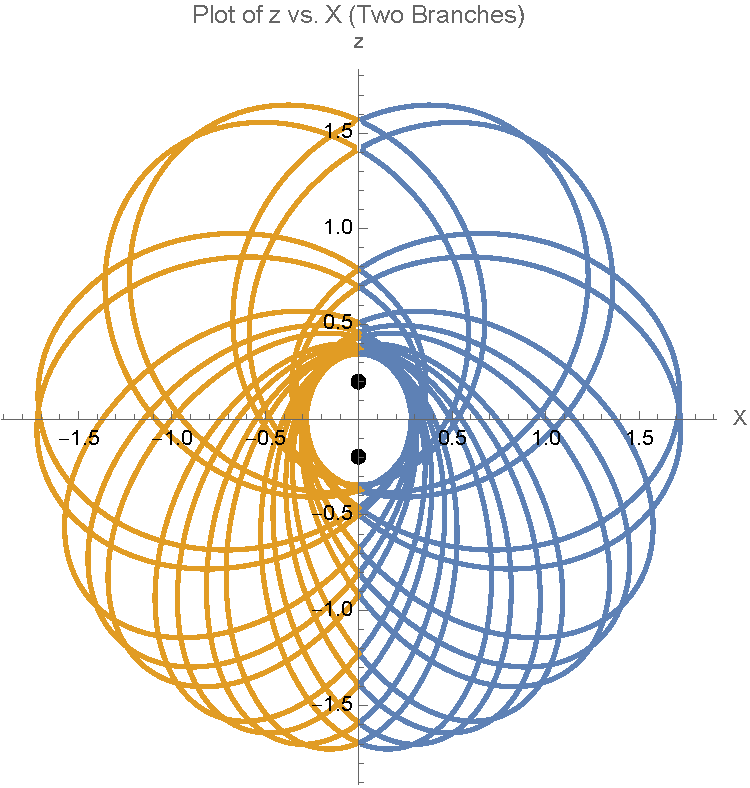
\includegraphics[width=\textwidth]{\detokenize{figures/plot figures first attempt/Class A1 figure 1 .pdf}}
        \caption{}
        \label{fig:Class_A1}
    \end{subfigure}
    \hfill
    \begin{subfigure}{0.48\textwidth}
        \centering
        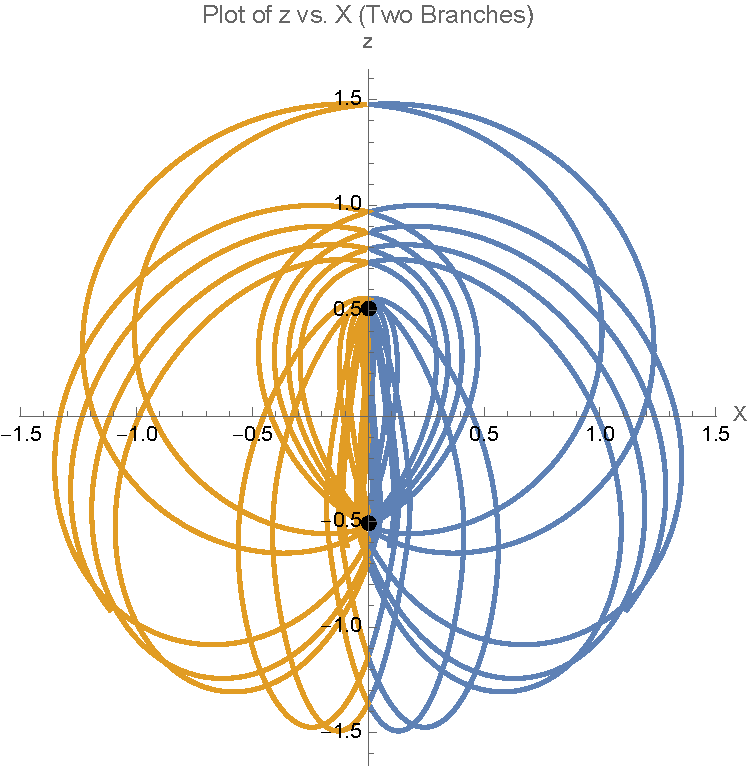
\includegraphics[width=\textwidth]{\detokenize{figures/plot figures first attempt/Class A2 figure 3.pdf}}
        \caption{}
        \label{fig:Class_A2}
    \end{subfigure}
    \vspace{-10pt} % Reduce vertical gap between figures
    \caption{Examples of Case I orbits via Mathematica code appendix \ref{Mathematica code}.}
    \label{fig:Class_A}
\end{figure}

\begin{figure}[H]
    \centering
    \begin{subfigure}{0.48\textwidth}
        \centering
        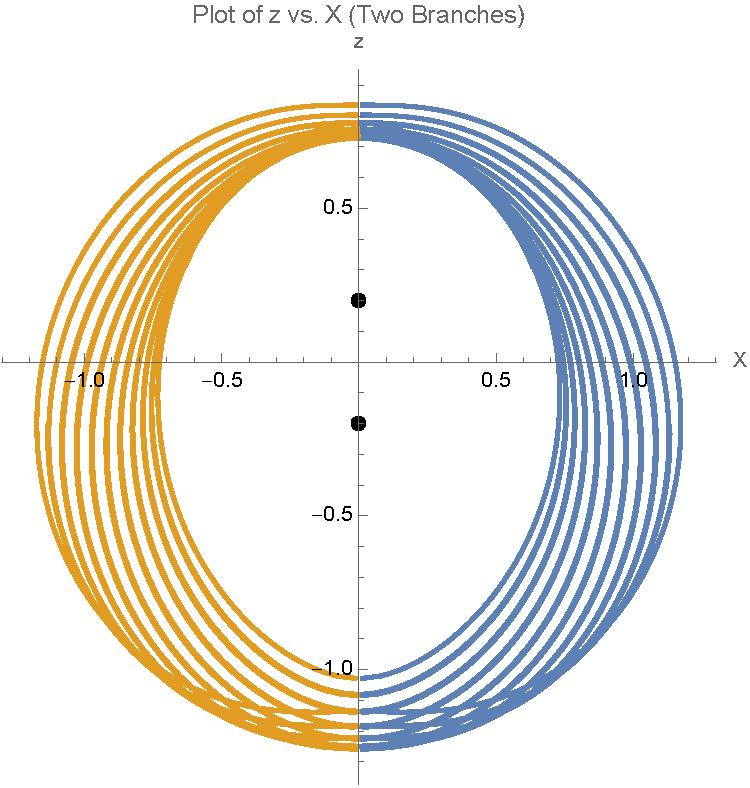
\includegraphics[width=\textwidth]{\detokenize{figures/plot figures first attempt/Class B1 figure 8.pdf}}
        \caption{}
        \label{fig:Class_B1}
    \end{subfigure}
    \hfill
    \begin{subfigure}{0.48\textwidth}
        \centering
        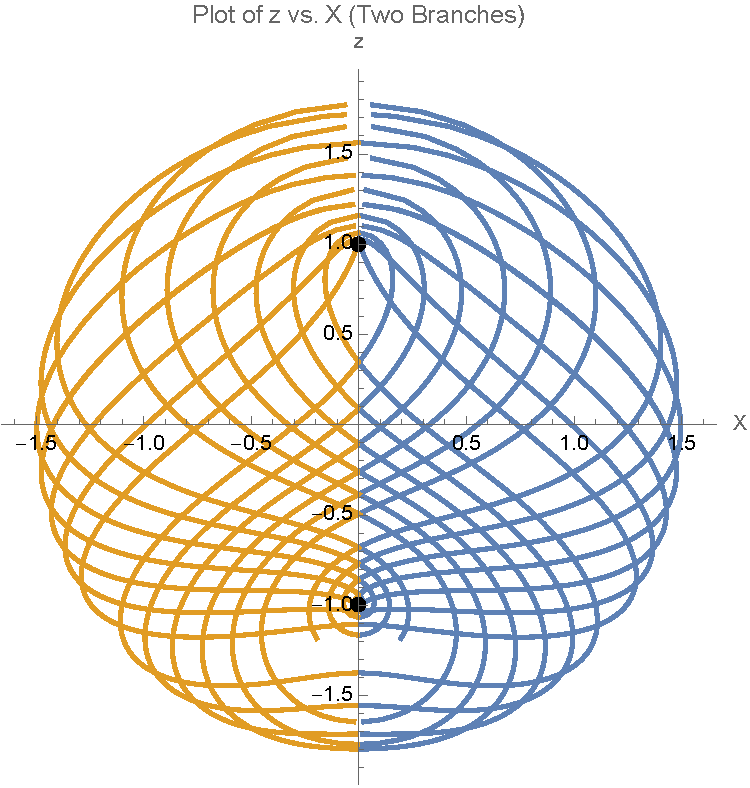
\includegraphics[width=\textwidth]{\detokenize{figures/plot figures first attempt/Class B2 figure 11.pdf}}
        \caption{}
        \label{fig:Class_B2}
    \end{subfigure}
    \vspace{-10pt} % Reduce vertical gap between figures
    \caption{Examples of Case II orbits via Mathematica code appendix \ref{Mathematica code}.}
    \label{fig:Class_B}
\end{figure}

\begin{remark}
    A few quick remarks here, First  recall that the coordinate system was defined as  
    \[
    r\sin{\theta} = x :=  \pm \sqrt{R^{2} - b^{2}}\sin{\sigma}, \quad r\cos{\theta} = z := R\cos{\sigma}.
    \]
    Thus, for each set of \(\sigma\) and \(S\), we obtain \((\pm x, z)\), hence the orange and blue colours in the plots in figures \ref{fig:Class_A} \& \ref{fig:Class_B}. This leads to us being limited to looking at symmetric orbit trajectories this is of course not the only possible orbits that could physically occur but the code created was limited to it. Second while it would be appropriate to include the time angle analysis for this problem we opted not to for the sake of space and because the primary interest was the solutions of trajectories.  
\end{remark}

\FloatBarrier  % Prevent figures from floating into the next section
\vspace{-5pt} % Reduce space before the section title


\section{Action-Angle Variables for Euler}

Having solved for the trajectories we now try determining the action-angle variables for this problem. First recall the two constants of motion: the Hamiltonian and the constant associated with \(p_{\sigma}\). Following the approach in Section~\ref{level set argument}, we focus on compact level sets, thus we get

\begin{equation}
\frac{1}{2}\left( \cfrac{p_{R}^{2}(R^{2}-b^{2})}{R^{2}-b^{2}\cos^{2}{\sigma}} + \cfrac{p_{\sigma}^{2}}{R^{2}-b^{2}\cos^{2}{\sigma}} \right) - \mu \cfrac{R+\beta b \cos{\sigma}}{R^{2}-b^{2}\cos^{2}{\sigma}}  = -\alpha^{2},
\end{equation}

\begin{equation}
\cfrac{p_{\sigma}^{2}}{2} - \alpha^{2}b^{2}\cos^{2}{\sigma}+\mu \beta b \cos{\sigma}  = \cfrac{C^{2}}{2}.
\end{equation}

Recognising that the Hamiltonian is time-independent, we apply Proposition \ref{Time independent HJ} and use an ansatz of the form $W(R,\sigma) = W_{R}(R) + W_{\sigma}(\sigma)$ in the Hamilton-Jacobi equation

\begin{equation}
H\left(q_{i},\pd{W}{q_{i}},t \right)  = -\alpha^{2}, \quad \text{where } p_{i} = \pd{W}{q_{i}}.
\end{equation}
Rearranging, we obtain

\begin{equation}
-\left(\pd{W_{R}}{R}\right)^{2}(R^{2}-b^{2})+2\mu R - 2\alpha^{2}R^{2} = \left(\pd{W_{\sigma}}{\sigma}\right)^{2}-2\mu \beta b \cos{\sigma} -2\alpha^{2}b^{2}\cos^{2}{\sigma}.
\end{equation}
Separating variables yields
\begin{subequations}
\begin{equation}
\pd{W_{R}}{R} = \sqrt{\cfrac{-2\alpha^{2}R^{2}+2\mu R - C^{2}}{R^{2}-b^{2}}},
\end{equation}
\begin{equation}
\pd{W_{\sigma}}{\sigma} = \sqrt{2\alpha^{2}b^{2}\cos^{2}{\sigma} + 2\mu \beta b \cos{\sigma} + C^{2}}.
\end{equation}
\end{subequations}
Thus, the action coordinates $I_{i}$ are given by

\begin{subequations}
\begin{equation}
I_{R} = \frac{1}{2\pi} \int_{\gamma_{R}} p_{R} \ dR = \frac{1}{2\pi}\int_{\gamma_{R}} \sqrt{\cfrac{-2\alpha^{2}R^{2}+2\mu R - C^{2}}{R^{2}-b^{2}}} \ dR,
\end{equation}
\begin{equation}
I_{\sigma} = \frac{1}{2\pi} \int_{\gamma_{\sigma}} p_{\sigma} \ d\sigma = \frac{1}{2\pi}\int_{\gamma_{\sigma}} \sqrt{2\alpha^{2}b^{2}\cos^{2}{\sigma} + 2\mu \beta b \cos{\sigma} + C^{2}} \ d\sigma.
\end{equation}
\end{subequations}

To evaluate these integrals, it is necessary to understand the integration contours in phase space. For \(I_{R}\), similar to \(I_{r}\) in the Kepler problem (see Section~\ref{Kepler Action angle}), we require that \(R\) have real roots in the numerator under the square root. Therefore, the contour is defined by integrating from \(R_{-}\) to \(R_{+}\) and multiplying by 2, where \(R_{\pm}\) are the roots of the quadratic. Note that, by our choice of coordinates, \(R > b\) so the denominator poses no issue. For \(I_{\sigma}\), the integral runs from 0 to \(\pi\) because \(\sigma \in [0,\pi]\).

\begin{remark}
Explicit solutions for these coordinates exist and can be found via \cite{byrd1971handbook} (equation 256.19). Although this evaluates to a combination of elliptic functions, we found it less useful for discussion in this report since it proved difficult to obtain the Hamiltonian via that approach. 
\end{remark}
We shall instead aim to look close to the kelper limit (i.e. $b$ is small) and seek a solution in terms of a series expansion via a Taylor series. To proceed, note that by our choice of coordinates \(R > b\). Therefore, since \(\frac{b}{R} < 1\) for small \(b\), we may expand the variable \(\frac{b^{2}}{R^{2}}\) in a Taylor series:

$$ \cfrac{1}{\sqrt{R^{2}-b^{2}}} = R^{-1}\left( 1- \frac{b^{2}}{R^{2}}\right)^{-\frac{1}{2}},$$
\begin{align}
    &= R^{-1} \sum_{k=0}^{\infty}\left( (-1)^{2k}\frac{(1+2k)!!}{2^{k} k!}\left(\frac{b^{2k}}{R^{2k}} \right)\right).
\end{align}
Substituting this series into the expression for $I_{R}$ yields
$$I_{R} = \frac{\alpha}{\pi}\int_{R_{-}}^{R_{+}} \sqrt{{-2R^{2}+\frac{2\mu}{\alpha^{2}} R - \frac{C^{2}}{\alpha^{2}}}} \left(\sum_{k=0}^{\infty}\cfrac{(1+2k)!!}{2^{k}k!}\cfrac{b^{2k}}{R^{2k+1}} \right) \ dR.$$
 Similar to the Kepler case, one may solve a complex contour integral that encloses the complement of the branch cut region from \(R_{-}\) to \(R_{+}\) (i.e., perform a residue calculation at \(R=0\) and as \(R\rightarrow \infty\)). However, we observe that pole as \(R\rightarrow \infty\) only contributes to leading order specifically, the \(\frac{1}{R}\) term in the expansion. In fact, the leading order term is the Kepler term, as it is independent of \(b\) and evaluates, as before, to
$$\frac{\alpha}{\pi}\int_{R_{-}}^{R_{+}}\cfrac{\sqrt{-2R^{2}+2\frac{\mu}{\alpha^{2}} R -\frac{C^{2}}{\alpha^{2}}}}{R}  \ dR = -C +\frac{\mu }{\sqrt{2\alpha^{2}}}. $$
 It is now sufficient to evaluate the residue of the \(k^{\text{th}}\) order term at \(R=0\) for a solution for \(I_{R}\). To that end, we employ the residue formula:
$$\text{Res}\left(I_{R},0\right) = \frac{1}{(2k)!}\lim_{R\rightarrow0} \left( \frac{(1+2k)!!b^{2k}}{2^{k}k!}\cfrac{d^{2k}}{dR^{2k}} \left[ R^{2k+1} \cfrac{\sqrt{-2R^{2}+2\frac{\mu}{\alpha^{2}} R -\frac{C^{2}}{\alpha^{2}}}}{R^{2k+1}} \right] \right) .$$
To determine the \(2k^{\text{th}}\) derivative, we use the general Leibniz rule:
\[
\frac{d^k}{dx^k} [f(x) g(x)] = \sum_{n=0}^{k} \binom{k}{n} f^{(k-n)}(x) g^{(n)}(x),
\]
for our purposes, we set
\[
f(R)=\sqrt{R-R_{-}} \quad \text{and} \quad g(R)=\sqrt{R_{+}-R}.
\]
The \(n^{\text{th}}\) derivative of \(f\) is then given by
\[
f^{(n)} = \frac{1}{2}\Bigl(\frac{1}{2}-1\Bigr)\cdots\Bigl(\frac{1}{2}-(n-1)\Bigr)(R-R_{-})^{\frac{1}{2}-n} = \frac{(-1)^{n-1}(2n-3)!!}{2^{n}}(R-R_{-})^{\frac{1}{2}-n}.
\]
Since this expression is only valid for \(n>1\), we may alternatively use the Gamma function as an analytic continuation of the factorial (see appendix \ref{Jacobi all functions}). In general, the relationship between the double factorial and the Gamma function is
\begin{equation}
z!! = \sqrt{\frac{2}{\pi}}\,2^{\frac{z}{2}}\Gamma\Bigl(\frac{z}{2}+1\Bigr).
\end{equation}
Thus $f^{(n)}$ and $g^{(n)}$ can be expressed as
$$f^{(n)} = \cfrac{(-1)^{n-1}\Gamma\left(n -\frac{1}{2}\right)}{\sqrt{\pi}}(R-R_{-})^{\frac{1}{2}-n},$$
$$g^{(n)} = \cfrac{-\Gamma\left(n -\frac{1}{2}\right)}{\sqrt{\pi}}(R_{+}-R)^{\frac{1}{2}-n}.$$
Returning to the residue calculation, we have
$$\text{Res}\left(I_{R},0\right) = \frac{1}{(2k)!}\frac{(1+2k)!!b^{2k}}{2^{k}k!}\lim_{R\rightarrow0} \left( \cfrac{d^{2k}}{dR^{2k}} \left[ {\sqrt{-R^{2}+2\frac{\mu}{\alpha^{2}} R -\frac{C^{2}}{\alpha^{2}}}} \right] \right) $$
$$ = \frac{1}{(2k)!}\frac{(1+2k)!!b^{2k}}{2^{k}k!} \sum_{n=0}^{2k}\binom{2k}{n}\cfrac{(-1)^{n}\Gamma\left(2k-n-\frac{1}{2}\right)\Gamma\left(n-\frac{1}{2}\right)}{\pi}(-R_{-})^{\frac{1}{2}-2k+n}(R_{+})^{\frac{1}{2}-n},$$
This gives the general expansion for \(I_{R}\):
\begin{equation}
\begin{split}
I_{R} &= -C + i\alpha \sum_{k=0}^{\infty} \frac{1}{(2k)!} 
\frac{(1+2k)!!b^{2k}}{2^{k}k!}  
\sum_{n=0}^{2k} \binom{2k}{n} \\
&\quad \times \frac{(-1)^{n} \Gamma\left(2k-n-\frac{1}{2}\right) 
\Gamma\left(n-\frac{1}{2}\right)}{\pi} \\
&\quad \times (-R_{-})^{\frac{1}{2}-2k+n} 
(R_{+})^{\frac{1}{2}-n}.
\end{split}
\end{equation}
Here, we do not worry about the factor \(i\) since we have the term \((-R_{-})^{\frac{1}{2}-2k+n}\) and we define the branch cut from \(R_{-}\) to \(R_{+}\).

Next, we shift our focus to the \(I_{\sigma}\) integrand. Making the substitution \(x = \cos\sigma\) yields
$$I_{\sigma} = \cfrac{\sqrt{2}\alpha}{2\pi}\int_{-1}^{1}\cfrac{\sqrt{x^{2}b^{2}+\frac{\mu\beta}{\alpha^{2}}  b x+\frac{C^{2}}{2\alpha^{2}}}}{\sqrt{1-x^{2}}} \ dx.$$
Since \(\sigma \in [0,\pi]\) implies \(|x|<1\) and near the Kepler limit \(b\) is small so that \(xb \ll 1\), we may expand in a Taylor series about 0. Using a procedure similar to that for \(I_{R}\) and letting \(x_{\pm}\) be the roots of the quadratic in the \(I_{\sigma}\) integrand, we have
$$\sqrt{x^{2}b^{2}+\frac{\mu \beta}{\alpha^{2}} + \frac{C^{2}}{2\alpha^{2}}} = \sqrt{(xb-x_{-})(xb-x_{+})}$$
$$ = \sum_{k=0}^{\infty}\frac{(xb)^{k}}{k!}\sum_{n=0}^{k}\binom{k}{n}\cfrac{(-1)^{k} \Gamma \left(k-n-\frac{1}{2} \right) \Gamma \left(n-\frac{1}{2} \right) }{\pi}(-x_{-})^{\frac{1}{2}-k+n}(-x_{+})^{\frac{1}{2}-n}.$$
Putting everything together, we obtain
$$ I_{\sigma}= \int_{-1}^{1}\sum_{k=0}^{\infty}\frac{(xb)^{k}}{k!\sqrt{1-x^{2}}}\sum_{n=0}^{k}\binom{k}{n}\cfrac{(-1)^{k} \Gamma \left(k-n-\frac{1}{2}\right) \Gamma \left(n-\frac{1}{2} \right) }{\pi}(-x_{-})^{\frac{1}{2}-k+n}(-x_{+})^{\frac{1}{2}-n} \ dx. $$
This is now aided by the following identity
\begin{equation}
  \int_{-1}^{1} \cfrac{x^{n}}{\sqrt{1-x^{2}}}=\begin{cases}
    \cfrac{\Gamma(n+\frac{1}{2})\sqrt{\pi}}{2\Gamma(n+1)}, & \text{if n is even}.\\
    0, & \text{if n is odd}.
  \end{cases}
\end{equation}
Since only even powers contribute, we may replace \(k\) by \(2k\), leading to the explicit series
$$I_{\sigma} = \frac{\sqrt{2}\alpha}{2\pi}\sum_{k=0}^{\infty}\cfrac{b^{2k}\sqrt{\pi}\Gamma \left(2k+\frac{1}{2}\right)}{2(2k)! \Gamma\left(2k+1\right)}\sum_{n=0}^{2k}\binom{2k}{n}\cfrac{ \Gamma \left(2k-n-\frac{1}{2}\right) \Gamma \left(n-\frac{1}{2} \right) }{\pi}(-x_{-})^{\frac{1}{2}-2k+n}(-x_{+})^{\frac{1}{2}-n}.$$
A quick sanity check shows that, at leading order (i.e., \(k=0\)) the value is \(C\), which is indeed the expected Kepler limit. In general, we have not been able to find the Hamiltonian as directly as in the Kepler case. However, we may extract \(H\) in a perturbative manner by considering terms up to \(\mathcal{O}(b^{2})\). The action coordinates are then given by
\begin{subequations}
    \begin{equation}\label{IR ham pert}
      I_{R}  = -C+\frac{\mu}{\sqrt{2\alpha^{2}}} -\frac{3b^{2}} {16}\left(\frac{-2\alpha^{2}}{C}+\frac{\mu^{2}}{C^{3}}\right) + \mathcal{O}(b^{4}),  
    \end{equation}
    \begin{equation}
      I_{\sigma} =  C + \frac{3b^{2}}{64}\left(\frac{2\alpha^{2}}{C}-\frac{\mu^{2}\beta^{2}}{C^{3}}\right) + \mathcal{O}(b^{4}).  
    \end{equation}
\end{subequations}
At this stage, one may proceed either via implicit inversion or by applying Lagrange's inversion theorem\footnote{See section 5.1 of chapter of \cite{wilf2005generatingfunctionology} for the general procedure, we do not include it in this report for the sake of space.}. In the implicit method, ignoring higher-order terms (i.e., \(\mathcal{O}(b^{4})\)) and rearranging for \(\alpha^{2}\) yields
$$
\alpha^{2} = \frac{C}{2} \left( \frac{64}{3b^{2}}(I_{\sigma} - C) + \frac{\mu^{2}\beta^{2}}{C^{3}} \right).
$$
For convenience, we define
$$X = \sqrt{2\alpha^2} = \sqrt{C \left( \frac{64}{3b^{2}}(I_{\sigma} - C) + \frac{\mu^{2}\beta^{2}}{C^{3}} \right)},$$
rearranging the expression for \(I_{R}\) in \eqref{IR ham pert} gives
\begin{equation*}
X = \frac{\mu}{I_{R} + C - \frac{3b^{2}}{16C} X^2 + \frac{3b^{2}}{16C^3} \mu^2},
\end{equation*}
and since \(X = \sqrt{2\alpha^2}\), we finally obtain
\begin{equation}
\alpha = \frac{1}{\sqrt{2}} \frac{\mu}{I_{R} + C - \frac{3b^{2}}{16C} X^2 + \frac{3b^{2}}{16C^3} \mu^2}.
\end{equation}
Recalling the level set \(H = -\alpha^{2}\), we then have
$$H = -\cfrac{\mu^{2}}{2(I_{R} + C - \frac{3b^{2}}{16C} X^2 + \frac{3b^{2}}{16C^3} \mu^2)^{2}}.$$
\begin{remark}
 At this stage, note that to obtain the Hamiltonian in terms of \(I_{R}\) and \(I_{\sigma}\) only, one must eliminate the \(C\) dependence. However, it is clear that in the limit \(b\to0\) (where \(I_{\sigma}\to C\)), the Kepler Hamiltonian is recovered.
\end{remark}
To find an explicit relation between \(H\) and the action variables \(I_i\), we first invert the relation for \(I_{\sigma}\) to express \(C\) as a function of \(I_{\sigma}\). Using the Lagrange inversion theorem, suppose
$$
I_\sigma = f(C) = C + b^{2}\,g(C),
$$
with \(b^{2}\) as a small parameter and
$$
g(C) = \frac{3}{64} \left(\frac{2\alpha^{2}}{C} - \frac{\mu^{2}\beta^{2}}{C^{3}}\right),
$$
then for $b=0$ we have the base solution $C=I_\sigma$. Assuming an expansion
$$
C = I_\sigma + c_1\,b^{2} + \mathcal{O}(b^4),
$$
we substitute back into the definition of $I_\sigma$ and match the coefficients order by order. At order $b^{2}$, one finds
$$
c_1 = -g(I_\sigma).
$$
Thus, the inverted series is
$$
C = I_\sigma - \frac{3b^{2}}{64}\left(\frac{2\alpha^{2}}{I_\sigma} - \frac{\mu^{2}\beta^{2}}{I_\sigma^{3}}\right) + \mathcal{O}(b^{4}).
$$
We may use the same idea once again by substituting $C$ in terms of $I_{\sigma}$ into \autoref{IR ham pert} and inverting for $\frac{\mu}{\sqrt{2\alpha^{2}}}$, we get
$$\cfrac{\mu}{\sqrt{2\alpha^{2}}} = (I_{R}+I_{\sigma}) - \frac{3b^{2}}{64}\left(\cfrac{2\mu^{2}}{I_{\sigma}(I_{\sigma}+I_{R})^{2}} - \cfrac{\mu^{2}\beta^{2}}{I_{\sigma}^{3}} \right) +\frac{3b^{2}}{16}\left( \cfrac{-2\mu^{2}}{I_{\sigma}(I_{\sigma}+I_{R})^{2}} + \cfrac{\mu^{2}}{I_{\sigma}^{3}}\right) + \mathcal{O}(b^{4}).$$
Now squaring and rearranging for $\frac{1}{\alpha^{2}}$ we obtain
 $$ \cfrac{1}{2\alpha^{2}} = \cfrac{(I_{R}+I_{\sigma})^{2}}{\mu^{2}} - 2(I_{R}+I_{\sigma})\frac{3b^{2}}{64}\left(\cfrac{10}{I_{\sigma}(I_{\sigma}+I_{R})^{2}} - \cfrac{(\beta^{2}+4)}{I_{\sigma}^{3}} \right) + \mathcal{O}(b^{4}), $$
for convenience we define the functions
$$ G_{0} = \cfrac{(I_{R}+I_{\sigma})^{2}}{\mu^{2}},$$
$$G_{1} = (I_{R}+I_{\sigma})\frac{3}{32}\left(\cfrac{10}{I_{\sigma}(I_{\sigma}+I_{R})^{2}} - \cfrac{(\beta^{2}+4)}{I_{\sigma}^{3}} \right) + \mathcal{O}(b^{4}). $$
Now ignoring higher order corrections and rearranging for $-\alpha^{2}$ we get
$$ -\alpha^{2} \approx \cfrac{-1}{2G_{0}}\left(1-b^{2}\cfrac{G_{1}}{G_{0}}\right)^{-1}.$$
Using a binomial expansion for small \(b^{2}\), we obtain
$$ H \defequal -\alpha^{2} \approx -\cfrac{\mu^{2}}{2(I_{R}+I_{\sigma})^{2}} -b^{2}\cfrac{G_{1}}{2G_{0}^{2}} + \mathcal{O}(b^{4}).$$
Where once again we've gotten the Kepler Hamiltonian in terms of some corrections (as $b \rightarrow 0$, $I_{\sigma} \rightarrow I_{\varphi}$). While the implicit expression in some sense is cleaner to obtain, the explicit one makes it clear that the action variables for the Euler Problem could be seen as a perturbation on the Kepler problem. In fact, one sees that just the $\mathcal{O}(b^{2})$ corrections were enough to lift the degeneracy of the orbital frequencies $\omega_{i}$'s displaying the complexity in contrast to the Kepler case. This was expected as we no longer in general had an ellipse as an orbit but rather had rotating ellipses and more complicated orbits as seen in figure \ref{fig:Class_A}.













\chapter{Conclusion}
In this report, motivated by the study of integrable systems in celestial mechanics \cite{o2008integrable}, we examined special cases of the two-body and three-body problems: the Kepler problem and the planar Euler problem. Beginning with an introduction to Hamiltonian mechanics and symplectic geometry, we established the framework for integrability through the Liouville-Arnold theorem.

We first analysed the Kepler problem, solving it using Lagrangian mechanics and ODE methods while verifying its integrability. This led naturally to the construction of action-angle variables, drawing on Classical Mechanics by Goldstein \cite{goldstein2002classical}. Our analysis confirmed that Keplerian orbits remain closed in configuration space due to degeneracies in orbital frequencies.

We then turned to the Planar Euler problem, where the system’s unique geometry justified the use of prolate spheroidal coordinates. By applying Möbius transformations and Jacobi elliptic functions, we derived explicit solutions and utilised Mathematica code to visualise symmetric orbits. The solutions exhibited diverse behaviours, including rotating ellipses and figure-eight-like trajectories, consistent with findings in \cite{o2008integrable}. However, a deeper exploration of these behaviours proved difficult due to the limitations of the code.

Finally, we constructed action variables for the Planar Euler problem, revealing how its Hamiltonian in action variables could be understood as a perturbation of the Keplerian case. The addition of the correction terms broke the degeneracy in the frequencies leading to precessing orbits, one of the defining differences between the two problems.

While our study confirmed the integrability of both systems, it also highlighted the richness of the Euler problem, where even first-order corrections to the Kepler limit introduced significant qualitative changes. Given more time, we would have pursued an exact solution for the Hamiltonian in action-angle variables, investigated the Vinti problem, and refined our orbit plotters to capture non-symmetric trajectories. These extensions would further illuminate the interplay between two problems deepening our understanding of celestial mechanics.






\appendix
\addcontentsline{toc}{chapter}{Appendix} % Optional: add to the table of contents

\chapter{Time Angle Relation Kelper}\label{appendix1}

This appendix is dedicated to solving the time angle relation in the Kelper problem. Recall the time angle relation(\autoref{2.9})and the solution for \(r\)(\autoref{2.12}):
\[
\frac{dt}{df} = \frac{r^2}{J}, \qquad
r = \frac{J^2/\mu}{1 + \sqrt{1 - \frac{2J^2\alpha^2}{\mu^2}}\, \cos(f+\omega_0)}.
\]
For consistency with \cite{o2008integrable}, we introduce the following constants:
\begin{equation}\label{2.16}
e := \sqrt{1 - \frac{2J^2\alpha^2}{\mu^2}},
\end{equation}
\begin{equation}\label{2.17}
a := \frac{J^2}{\mu(1-e^2)},
\end{equation}
\begin{equation}\label{2.18}
n := \sqrt{\frac{\mu}{a^3}}.
\end{equation}
With these definitions, \autoref{2.9} becomes
\begin{equation}\label{2.19}
n\,\frac{dt}{df} = \frac{(1-e^2)^{3/2}}{(1+e\cos f)^2}.
\end{equation}
To integrate \autoref{2.19}, note that
\[
\frac{d}{df}\left[\frac{e\sin f}{1+e\cos f}\right] 
=\frac{e^2+e\cos f}{(1+e\cos f)^2}
=\frac{1}{1+e\cos f} - \frac{1-e^2}{(1+e\cos f)^2}.
\]
Multiplying both sides by \(\sqrt{1-e^2}\) gives
\begin{equation}\label{2.20}
\frac{(1-e^2)^{3/2}}{(1+e\cos f)^2} 
= \frac{\sqrt{1-e^2}}{1+e\cos f} - \frac{d}{df}\left[\frac{e\sqrt{1-e^2}\sin f}{1+e\cos f}\right].
\end{equation}
To integrate the first term on the right, define the auxiliary variable \(\chi\) by
\begin{equation}\label{2.21}
\tan\chi = \frac{\sqrt{1-e^2}\sin f}{e+\cos f}.
\end{equation}
One may verify that
\[
\cos\chi = \frac{e+\cos f}{1+e\cos f}, \qquad
\sin\chi = \frac{\sqrt{1-e^2}\sin f}{1+e\cos f}.
\]
Differentiating \autoref{2.21} with respect to \(f\) yields
\begin{equation}\label{2.22}
\chi' = \frac{\sqrt{1-e^2}}{1+e\cos f}.
\end{equation}
Thus,
\begin{equation}\label{2.23}
\int \frac{\sqrt{1-e^2}}{1+e\cos f}\,df = \chi = \arctan\left[\frac{\sqrt{1-e^2}\sin f}{e+\cos f}\right].
\end{equation}
Combining \autoref{2.19}, \autoref{2.20}, and \autoref{2.23}, we obtain the integrated form:
\begin{equation}\label{2.24}
M := n(t-t_0) = \arctan\left[\frac{\sqrt{1-e^2}\sin f}{e+\cos f}\right] - \frac{e\sqrt{1-e^2}\sin f}{1+e\cos f},
\end{equation}
where \(t_0\) is an integration constant and \(M\) is known as the mean anomaly \cite{o2008integrable}.


\chapter{Special Functions }\label{Elliptic functions}
This appendix is dedicated to a concise overview of the special functions used throughout this report. Rather than providing a comprehensive introduction, we highlight key definitions, properties, and identities that play a central role in our analysis.

\section{Jacobi Elliptic Functions}
This section is primarily based on Chapter 16 of \cite{abramowitz1968handbook}. The Jacobi elliptic functions form a class of doubly periodic meromorphic functions that generalize the trigonometric functions to the setting of elliptic curves. They depend on the elliptic modulus \(k\) and its complementary modulus \(k'\), where
\[
k'^2 = 1 - k^2,
\]
or equivalently,
\[
k^2 + k'^2 = 1.
\]

\begin{remark}
In order to maintain consistency with \cite{o2008integrable}, we have modified the notation originally used in \cite{abramowitz1968handbook}.
\end{remark}

The complete elliptic integrals of the first kind are defined by
\begin{equation}\label{eq:K}
K(k) = \int_0^{\pi/2} \frac{d\theta}{\sqrt{1 - k^2 \sin^2 \theta}},
\end{equation}
\begin{equation}\label{eq:Kprime}
iK'(k) = i\int_0^{\pi/2} \frac{d\theta}{\sqrt{1 - k'^2 \sin^2 \theta}}.
\end{equation}
These integrals represent the real and imaginary quarter-periods, respectively, and they establish a rectangular lattice structure in the complex plane.

\subsection{Definition and Fundamental Identities}
The Jacobi elliptic functions are introduced via the \textit{amplitude} function \(\varphi\) defined by
\begin{equation}\label{eq:amplitude}
u = \int_0^{\varphi} \frac{d\theta}{\sqrt{1 - k^2 \sin^2 \theta}},
\end{equation}
where \(u\) is the \textit{elliptic argument}. The three primary Jacobi elliptic functions are then defined as follows:
\begin{align}\label{Jacobi all functions}
\text{sn}(u;k) &= \sin\varphi,
\\
\text{cn}(u;k) &= \cos\varphi,
\\
\text{dn}(u;k) &= \sqrt{1 - k^2 \sin^2 \varphi}. 
\end{align}

Among the many identities these functions satisfy, the following are particularly useful:
\begin{subequations}\label{eq:jacobi_identities}
\begin{align}
\text{cn}\bigl[u \pm K(k); k\bigr] &= \mp k'\,\frac{\text{sn}(u; k)}{\text{dn}(u; k)}, \label{Jacobi cn} \\
\text{sn}\bigl[u \pm K(k); k\bigr] &= \pm\frac{\text{cn}(u; k)}{\text{dn}(u; k)}. \label{Jacobi sn}
\end{align}
\end{subequations}

\section{Gamma Function}
The Gamma function provides an analytic continuation of the factorial function to the complex plane. For non-negative integers \(n\), the factorial is defined by
\[
n! = n \cdot (n-1) \cdot (n-2) \cdots 1, \quad \text{with} \quad 0! = 1.
\]
A related integral representation is given by
\[
I(n) = \int_{0}^{\infty} e^{-t} t^{n} \, dt.
\]
To extend this definition to complex numbers \(z\) (with \(\Re(z)>0\) for convergence), we define the Gamma function by
\[
\Gamma(z) = \int_{0}^{\infty} e^{-t}t^{\,z-1}\,dt, \quad \Re(z)>0.
\]
This definition satisfies the recurrence relation
\[
\Gamma(z+1) = z\,\Gamma(z),
\]
so that for natural numbers, \(\Gamma(n+1) = n!\).

Some key identities involving the Gamma function are:
\begin{itemize}
    \item \(\Gamma\!\left(\frac{1}{2}\right) = \sqrt{\pi}\),
    \item The double factorial for \(z\) can be expressed as
    \[
    z!! = \sqrt{\frac{2}{\pi}}\,2^{\frac{z}{2}}\Gamma\!\Bigl(\frac{z}{2}+1\Bigr).
    \]
\end{itemize}
\chapter{Explicit Procedure}\label{Ganalysis}

This appendix is to work out the intermediary steps for the Möbius transformation in the Euler problem. We begin by considering equations of the form
\[
\frac{\Lambda^{2}}{C^{2}}\, {y'}^{2} = (1-y^{2})\Bigl[(1-d^{2}) + 2sy + qy^{2}\Bigr],
\]
for the variables \(S\) and \(v\) (with \(R\) related to \(v\) as defined above). It is convenient to transform the above equation (see \autoref{genericeq}) into one of the form
\begin{equation}\label{rquired}
\frac{\Lambda^{2}}{C^{2}}\, {Y'}^{2} = (1-Y^{2})\Bigl(A + BY^{2}\Bigr),
\end{equation}
since we have a free parameter \(\Lambda\) (recall that \(\Lambda\) has units of angular momentum) which can be chosen so that the solutions are expressed in terms of elliptic functions. For example, one obtains
\begin{subequations}
    \begin{equation}
        {Y'}^{2} = (1-Y^{2})(1-k_{1}^{2}Y^{2})
        \quad \Longrightarrow \quad Y = \operatorname{sn}[f+f_{0}:k_{1}],
    \end{equation}
    \begin{equation}
        {Y'}^{2} = (1-Y^{2})\Bigl(1-k_{2}^{2}(1-Y^{2})\Bigr)
        \quad \Longrightarrow \quad Y = \operatorname{cn}[f+f_{0}-K_{2}:k_{2}],
    \end{equation}
\end{subequations}
where \(K_{2}\) is the quarter period of the Jacobi elliptic function of modulus \(k_{2}\).

\begin{remark}
We do not provide a rigorous definition of these elliptic functions here; see \autoref{Jacobi all functions} for further details and useful relationships.
\end{remark}
It turns out that a Möbius transformation achieves the desired form. To show this explicitly, note that the generic equation (\autoref{genericeq}) contains two quadratic factors on the right-hand side. Our goal is to recast these so that both quadratic terms become linear. We proceed as follows.

\noindent First, consider the factor \(1-y^{2}\). Write it as
\[
(1-y^{2}) = J^{2}\Bigl[(1-\delta y)^{2} - (y-\delta)^{2}\Bigr] = J^{2}(1-\delta^{2})(1-y^{2}),
\]
which requires the arbitrary constants \(J\) and \(\delta\) to satisfy
\begin{equation}\label{7.2}
J^{2}(1-\delta^{2}) = 1.
\end{equation}
Next, for the second factor in \autoref{genericeq}, set
\[
(1-d^{2}) + 2sy + qy^{2} = J^{2}\Bigl[A(1-\delta y)^{2} + B(y-\delta)^{2}\Bigr],
\]
which expands to
\[
J^{2}\Bigl[(A+B\delta^{2}) - 2\delta(A+B)y + (A\delta^{2}+B)y^{2}\Bigr].
\]
To obtain the form in \autoref{rquired}, we impose the following restrictions:
\begin{subequations}
    \begin{equation}\label{a}
    J^{2}(A+B\delta^{2}) = 1-d^{2},
    \end{equation}
    \begin{equation}\label{b}
    J^{2}\delta(A+B) = -s,
    \end{equation}
    \begin{equation}\label{c}
    J^{2}(A\delta^{2}+B) = q.
    \end{equation}
\end{subequations}
Adding \autoref{a} and \autoref{c} yields
\begin{equation}\label{d}
J^{2}(1+\delta^{2})(A+B) = (1-d^{2})+q,
\end{equation}
while subtracting \autoref{c} from \autoref{a} gives
\begin{equation}\label{e}
J^{2}(1-\delta^{2})(A-B) = (1-d^{2})-q.
\end{equation}
Multiplying \autoref{b} by 2 and adding to \autoref{d} leads to
\begin{equation}\label{f}
J^{2}(1+\delta)^{2}(A+B) = (1-d^{2})-2s+q,
\end{equation}
and subtracting the same from \autoref{d} results in
\begin{equation}\label{g}
J^{2}(1-\delta^{2})(A+B) = (1-d^{2})+2s+q.
\end{equation}
Dividing \autoref{g} by \autoref{f} and defining a new parameter \(\rho\) for convenience, we set
\begin{equation}\label{h}
\rho^{2} := \Bigl(\frac{1-\delta}{1+\delta}\Bigr)^{2} = \frac{(1-d^{2})+2s+q}{(1-d^{2})-2s+q}.
\end{equation}
Thus,
\begin{equation}\label{ij}
\rho = \sqrt{\frac{(1-d^{2})+2s+q}{(1-d^{2})-2s+q}} \quad \Longrightarrow \quad \frac{1-\delta}{1+\delta} = \pm \rho.
\end{equation}
Requiring \(\rho \to 1\) as \(\delta \to 0\) selects the positive sign, so that
\begin{equation}\label{k}
\delta = \frac{1-\rho}{1+\rho}.
\end{equation}
Then,
\begin{equation}\label{l}
1-\delta^{2} = \frac{4\rho}{(1+\rho)^{2}}, \qquad J^{2} = \frac{1+\rho^{2}}{4\rho}.
\end{equation}
It follows from \autoref{h} that
\begin{equation}\label{m}
1-\rho^{2} = -\frac{4s}{(1-d^{2})-2s+q}.
\end{equation}
Using \autoref{h} and \autoref{ij}, we write
\[
(1+\rho)^{2} = 1+\rho^{2}+2\rho,
\]
and further,
\begin{equation}\label{n}
(1+\rho)^{2} = 2 \left[ \frac{(1-d^{2})+q + \sqrt{\bigl[(1-d^{2})-2s+q\bigr]\bigl[(1-d^{2})+2s+q\bigr]}}{(1-d^{2})-2s+q} \right].
\end{equation}
Next, observe that
\begin{equation}\label{o}
\bigl[(1-d^{2})-2s+q\bigr]\bigl[(1-d^{2})+2s+q\bigr] = \bigl[(1-d^{2})+q\bigr]^{2}\left[1-\frac{4s^{2}}{[(1-d^{2})+q]^{2}}\right].
\end{equation}
Define a parameter \(h\) by
\begin{equation}\label{p}
(1-2h)^{2} = 1 - \frac{4s^{2}}{[(1-d^{2})+q]^{2}},
\end{equation}
so that
\begin{subequations}
    \begin{equation}\label{hcoeff1}
    h = \frac{1}{2}\Biggl[1 - \sqrt{1 - \frac{4s^{2}}{[(1-d^{2})+q]^{2}}}\Biggr],
    \end{equation}
    \begin{equation}\label{hcoeff2}
    1-h = \frac{1}{2}\Biggl[1 + \sqrt{1 - \frac{4s^{2}}{[(1-d^{2})+q]^{2}}}\Biggr].
    \end{equation}
\end{subequations}
Then, from \autoref{o},
\begin{equation}\label{q}
\sqrt{\bigl[(1-d^{2})-2s+q\bigr]\bigl[(1-d^{2})+2s+q\bigr]} = \bigl[(1-d^{2})+q\bigr](1-2h).
\end{equation}
Recall \autoref{n}, which can now be written in terms of \(h\) as
\begin{equation}\label{r}
(1+\rho)^{2} = \frac{4(1-h)\bigl[(1-d^{2})+q\bigr]}{(1-d^{2})-2s+q}.
\end{equation}
Returning to \autoref{k} and using \autoref{m} and \autoref{r}, we obtain
\begin{equation}\label{7.5}
\delta = \frac{1-\rho}{1+\rho} = \frac{1-\rho^{2}}{(1+\rho^{2})^{2}} = -\frac{s}{\bigl[(1-d^{2})+q\bigr](1-h)}.
\end{equation}
From \autoref{f}, introducing \(J^{2}\) from \autoref{7.2}, we have
\[
(1-d^{2})-2s+q = \frac{(1+\delta)^{2}}{1-\delta^{2}}(A+B)
= \frac{A+B}{\rho},
\]
so that
\[
A+B = \rho\Bigl[(1-d^{2})-2s+q\Bigr] = \sqrt{\bigl[(1-d^{2})-2s+q\bigr]\bigl[(1-d^{2})+2s+q\bigr]}.
\]
Using \autoref{q}, this gives
\[
A+B = \bigl[(1-d^{2})+q\bigr](1-2h).
\]
Similarly, from \autoref{e},
\[
A-B = (1-d^{2})-q.
\]
Solving these yields
\begin{subequations}
    \begin{equation}\label{7.8}
    A = (1-d^{2})(1-h) - hq,
    \end{equation}
    \begin{equation}
    B = -h(1-d^{2}) + q(1-h).
    \end{equation}
\end{subequations}
With \(h\) determined in terms of \(d\), \(s\), and \(q\) from \autoref{hcoeff1}, and with \(\delta\), \(A\), and \(B\) given by \autoref{7.5} and \autoref{7.8} respectively (and \(J^{2}\) determined by \autoref{7.2}), all the quantities are now fully determined algebraically.

\noindent Finally, putting all factors together, we have
\[
\frac{\Lambda^{2}}{C^{2}}\, {y'}^{2} = J^{4}\Bigl[(1-\delta y)^{2} - (y-\delta)^{2}\Bigr]
\Bigl[A(1-\delta y)^{2} + B(y-\delta)^{2}\Bigr].
\]
This can be rewritten as
\[
\frac{\Lambda^{2}}{C^{2}} \left[ \frac{y'}{J^{2}(1-\delta y)^{2}} \right]^{2} = \left[ 1- \left( \frac{y-\delta}{1-\delta y}\right)^{2}\right]
\left[A+B\left( \frac{y-\delta}{1-\delta y} \right)^{2}\right].
\]
We now identify the Möbius transformation
\begin{equation}
Y = \frac{y-\delta}{1-\delta y} \quad \text{or equivalently} \quad y = \frac{Y+\delta}{1+\delta Y},
\end{equation}
so that
\[
{Y'}^{2} = \frac{y'}{J^{2}(1-\delta y)^{2}}.
\]
In terms of \(Y\), the equation becomes
\[
\frac{\Lambda^{2}}{C^{2}}\, {Y'}^{2} = (1-Y^{2})\Bigl[A+B\,Y^{2}\Bigr],
\]
which is exactly the desired form given in \autoref{rquired}.
 

\chapter{Mathematica Code}\label{Mathematica code}

The following Mathematica code was used to plot orbits for the planar Euler problem.

\begin{verbatim}
(* Case I *)
(* Variables set up *)
B = 0.75;
e = 1.4;
b = 2.2;

(* Relations to main parameters *)
g = Sqrt[e^2 + B^2 - 1];

eeta[b_, e_] := b/(1 - e^2);
p = (1 - e^2);

f = eeta[b, e];

d0[f_, e_] := 
  2/((1 - f^2*(1 - e^2)) + Sqrt[(1 - f^2*(1 + e^2))^2 - 4*f^4*e^2]);
deltaV = f^2*d0[f, e];
eStar = e*((1 + f^2*d0[f, e])/(1 + f^2*d0[f, e]*e^2));

kS1 = Sqrt[((1 - f^2*(1 - e^2) - 
       Sqrt[(1 + f^2*(1 - e^2))^2 - 4*f^2*B^2]))/(1 - f^2*(1 - e^2) + 
      Sqrt[(1 + f^2*(1 - e^2))^2 - 4*f^2*B^2])];
deltaS = (-2*f*B)/(1 + f^2*(1 - e^2) + 
     Sqrt[(1 + f^2*(1 - e^2))^2 - 4*f^2*B^2]);
kv = Sqrt[f^2*e^2*(1 + 2*f^2 + f^4*(2 + e^2))];
jv = Sqrt[(1 - f^2*(1 - e^2) + 
      Sqrt[(1 - f^2*(1 - e^2))^2 - 4*f^2*e^2])/(2*
      Sqrt[(1 + f^2*(1 - e^2))^2 - 4*f^2*e^2])];
kS0 = ((2*Sqrt[b*g] - Sqrt[(b + g)^2 - B^2])/(2*Sqrt[b*g] + 
      Sqrt[(b + g)^2 - B^2]));
deltaSS = (((-b - g)*(b + B - g))/((b + g)^2 + B*(b - g) + 
      2*Sqrt[b*g*((b + g)^2 - B^2)]));

deltaR = -(((b + e)*(1 - (b - e)))/((b + e)^2 - (b - e) + 
       2*Sqrt[b*e]*Sqrt[(b + e)^2 - 1]));
kR = ((2*Sqrt[b*e] - Sqrt[(b + e)^2 - 1])/(2*Sqrt[b*e] + 
      Sqrt[(b + e)^2 - 1]));

(*for 1-e<=b<=B-g*)
jr1 = Sqrt[(2*Sqrt[b*e] + 
       Sqrt[(b + e)^2 - 1])^2/(2*((1 - e^2 + b^2) + 
        Sqrt[(1 - e^2 + b^2)^2 - 4*b^2*B^2]))];
(*for B-g<=b<=1+e*)
jr0 = (2*Sqrt[b*e] + Sqrt[(b + e)^2 - 1])/(2*Sqrt[b*g] + 
     Sqrt[(b + g)^2 - B^2]);

(* Case A *)
(* Define R as a function of f_v using dn and cn elliptic functions *)
R[f_, p_, deltaV_, eStar_, kv_, jv_] := 
  p*(JacobiDN[f*jv, kv] + 
      deltaV*JacobiCN[f*jv, kv])/(JacobiDN[f*jv, kv] + 
      eStar*JacobiCN[f*jv, kv]);

R2[f_, p_, deltaR_, b_, e_, kR_, jr_] := 
  0.5*(1 - b + 
      e)*((JacobiCN[f*jr, kR] + 
        deltaR*JacobiDN[f*jr, kR])/(JacobiDN[f*jr, kR] + 
        deltaR*JacobiCN[f*jr, kR])) + 0.5*(1 + b + e);

(* Define conditional R function *)
Rconditional[f_, p_, deltaV_, eStar_, kv_, jv_, deltaR_, b_, e_, kR_, 
   jr1_, jr0_] := 
  Which[0 <= b <= 1 - e, R[f, p, deltaV, eStar, kv, jv], 
   1 - e <= b <= B - g, R2[f, p, deltaR, b, e, kR, jr1], 
   B - g <= b <= 1 + e, R2[f, p, deltaR, b, e, kR, jr0]];

(* Define \[Sigma] as a function of f using sn elliptic function *)
sigma[f_, fS0_, kS1_, deltaS_] := 
  ArcCos[(JacobiSN[f + fS0, kS1] + deltaS)/(1 + 
      deltaS*JacobiSN[f + fS0, kS1])];

sigma2[f_, fS0_, kS0_, deltaSS_] := 
  ArcCos[(((1 + deltaSS)*b + (1 - deltaSS)*(B - g))*
       JacobiSN[f + fS0, 
        kS0] + ((1 + deltaSS)*b - (1 - deltaSS)*(B - g)))/(1 + 
      deltaSS*JacobiSN[f + fS0, kS0])];

(* Define conditional sigma function *)
sigmaconditional[f_, fS0_, kS1_, deltaS_, kS0_, deltaSS_] := 
  Which[0 <= b <= B - g, sigma[f, fS0, kS1, deltaS], b >= B - g, 
   sigma2[f, fS0, kS0, deltaSS]];

(* Set parameters for \[Sigma] *)
fS0 = 0.5; (* Offset for elliptic function *)

(* Define X and z in terms of R and \[Sigma], including both branches for X *)
XPlus[f_] := 
  Sqrt[Rconditional[f, p, deltaV, eStar, kv, jv, deltaR, b, e, kR, 
       jr1, jr0]^2 - b^2]*
   Sin[sigmaconditional[f, fS0, kS1, deltaS, kS0, deltaSS]];
XMinus[f_] := -Sqrt[
     Rconditional[f, p, deltaV, eStar, kv, jv, deltaR, b, e, kR, jr1, 
        jr0]^2 - b^2]*
   Sin[sigmaconditional[f, fS0, kS1, deltaS, kS0, deltaSS]];
z[f_] := 
  Rconditional[f, p, deltaV, eStar, kv, jv, deltaR, b, e, kR, jr1, 
    jr0]*Cos[sigmaconditional[f, fS0, kS1, deltaS, kS0, deltaSS]];

(* Define specific points to be included *)
specificPoints = {{0, b}, {0, -b}};

(* Plot z vs. X for both branches of X as a parametric plot by varying f *)
Show[ParametricPlot[{{XPlus[f], z[f]}, {XMinus[f], z[f]}}, {f, 0, 
   25 Pi}, PlotRange -> All, 
  PlotLabel -> "Plot of z vs. X (Two Branches)", 
  AxesLabel -> {"X", "z"}, AspectRatio -> 1, 
  PlotStyle -> {LightOrangeOrange, LightBlueBlue}], 
 ListPlot[specificPoints, PlotStyle -> {Black, PointSize[Large]}]]
\end{verbatim}

\begin{verbatim}
    (*Case II parameters*)B = 0;
e = 0.7005;
b = 0.9;

(*Relations to main parameters*)
g = Sqrt[e^2 + B^2 - 1];

eeta[b_, e_] := b/(1 - e^2);
p = (1 - e^2);

f = eeta[b, e];
ps = p[e];
d0[f_, e_] := 
  2/((1 - f^2*(1 - e^2)) + Sqrt[(1 - f^2*(1 + e^2))^2 - 4*f^4*e^2]);
deltaV = f^2*d0[f, e];
eStar = e*((1 + f^2*d0[f, e])/(1 + f^2*d0[f, e]*e^2));
deltaR = -(((b + e)*(1 - (b - e)))/((b + e)^2 - (b - e) + 
       2 Sqrt[b*e]*Sqrt[(b + e)^2 - 1]));
kR = ((2*Sqrt[b*e] - Sqrt[(b + e)^2 - 1])/(2*Sqrt[b*e] + 
      Sqrt[(b + e)^2 - 1]));

kS2 = 0.5 - 
   0.5*((1 - f^2*(1 - e^2))/(Sqrt[(1 + f^2*(1 - e^2))^2 - 4*f^2*B^2]));
deltaS = (-2*f*B)/(1 + f^2 (1 - e^2) + 
     Sqrt[(1 + f^2 (1 - e^2))^2 - 4*f^2*B^2]);
kv = Sqrt[f^2*e^2 (1 + 2*f^2 + f^4*(2 + e^2))];
jv = Sqrt[(1 - f^2 (1 - e^2) + 
      Sqrt[(1 - f^2 (1 - e^2))^2 - 4*f^2*e^2])/(1 - f^2 (1 - e^2) + 
      Sqrt[(1 + f^2 (1 - e^2))^2 - 4*f^2*e^2])];
jr2 = 0.5*
   Sqrt[(2*Sqrt[b*e] + 
        Sqrt[(b + e)^2 - 1])^2/(Sqrt[(1 - e^2 + b^2)^2 - 4*b^2*B^2])];

(*Case B*)
(*Define R as a function of f_v using dn and cn elliptic functions*)
(*for 0<=b<=1-e*)
R[f_, p_, deltaV_, eStar_, kv_, jv_] := 
  p*(JacobiDN[f*jv, kv] + 
      deltaV*JacobiCN[f*jv, kv])/(JacobiDN[f*jv, kv] + 
      eStar*JacobiCN[f*jv, kv]);

(*for 1-e<=b<=1+e*)
R2[f_, p_, deltaR_, b_, e_, kR_, jr2_] := 
  0.5*(1 - b + 
      e)*((JacobiCN[f*jr2, kR] + 
        deltaR*JacobiDN[f*jr2, kR])/(JacobiDN[f*jr2, kR] + 
        deltaR*JacobiCN[f*jr2, kR])) + 0.5*(1 + b + e);

(*Define conditional R function*)
Rconditional[f_, p_, deltaV_, eStar_, kv_, jv_, deltaR_, b_, e_, kR_, 
   jr2_] := 
  Which[0 <= b <= 1 - e, R[f, p, deltaV, eStar, kv, jv], 
   1 - e <= b <= 1 + e, R2[f, p, deltaR, b, e, kR, jr2]];

(*Define \[Sigma] as a function of f using sn elliptic function*)
sigma[f_, fS0_, kS2_, deltaS_] := 
  ArcCos[((Sqrt[1 - kS2^2])*JacobiSN[f + fS0, kS2] + 
      deltaS*JacobiDN[f + fS0, kS2])/(JacobiDN[f + fS0, 
       kS2] + (Sqrt[1 - kS2^2])*deltaS*JacobiSN[f + fS0, kS2])];

(*Set parameters for \[Sigma]*)
fS0 = 0; (*Offset for elliptic function*)

(*Define X and z in terms of R and \[Sigma],including both branches \
for X*)
XPlus[f_] := 
  Sqrt[Rconditional[f, p, deltaV, eStar, kv, jv, deltaR, b, e, kR, 
       jr2]^2 - b^2]*Sin[sigma[f, fS0, kS2, deltaS]];
XMinus[f_] := -Sqrt[
     Rconditional[f, p, deltaV, eStar, kv, jv, deltaR, b, e, kR, 
        jr2]^2 - b^2]*Sin[sigma[f, fS0, kS2, deltaS]];
z[f_] := 
  Rconditional[f, p, deltaV, eStar, kv, jv, deltaR, b, e, kR, jr2]*
   Cos[sigma[f, fS0, kS2, deltaS]];

(*Define specific points to be included*)
specificPoints = {{0, b}, {0, -b}};

(*Plot z vs.X for both branches of X as a parametric plot by varying \
f*)
Show[ParametricPlot[{{XPlus[f], z[f]}, {XMinus[f], z[f]}}, {f, 0, 
   25 Pi}, PlotRange -> All, 
  PlotLabel -> "Plot of z vs. X (Two Branches)", 
  AxesLabel -> {"X", "z"}, AspectRatio -> 1, 
  PlotStyle -> {LightOrangeOrange, LightBlueBlue}], 
 ListPlot[specificPoints, PlotStyle -> {Black, PointSize[Large]}]]
\end{verbatim}


% \bibliographystyle{amsalpha} % Example bibliography style
%\bibliography{references}   % Use your bibliography file
\printbibliography % Prints the bibliography
\addcontentsline{toc}{chapter}{Bibliography}





\end{document}
